
\subsection{N-band imaging recipes}
\label{ssec:recipes_img_n}
%------------------------------------------------------------------------------------------------------------------
\subsubsection{\REC*{metis_n_img_flat}:  Flatfielding}
\label{n_img_flatfield}
\label{rec:n_img_flatfield}
\label{sssec:n_img_flatfield}
\label{n_img_flat}
\label{rec:n_img_flat}
\label{sssec:n_img_flat}
\label{metis_n_img_flat}
\label{rec:metis_n_img_flat}
\label{sssec:metis_n_img_flat}

The purpose of the flat-field calibration is to determine
pixel-to-pixel gain variations and large scale illumination variations
(due to inhomogeneities of optical elements in the telescope or
instrument). Calibration frames are obtained either during day time
using the black-body lamp of the \ac{WCU} (internal flats) or by taken
images of the twilight sky (twilight flats). Advantages and
disadvantages of the two types of flat are discussed in
\cite{METIS-calibration_plan}.

MIR detectors are typically unstable in that they show gain
fluctuations on rather short time scales, hence science exposures may
have a different flat-field structure from those captured by the
calibration flats.  The GeoSnap detector is more linear
than the H2RG detectors, but should be flat-fielded anyway.
N-band flat fields will also be taken for quality control and monitoring purposes.

Since the operational concept for twilight flats needs to be refined
during commissioning at the telescope, the current recipe design is
primarily valid for internal flats.

This recipe creates a master flat for the GeoSnap detector (N-band
imaging) from lamp or sky images matched by various setup parameters
as detailed below.  A set of internal flats includes a number of
exposures with \CODE{LAMP OFF}, which will be used for dark
subtraction. For twilight flats a master dark will be subtracted. The
master flat is obtained by the slope of a linear fit of the pixel
values against the illumination level of the exposures.

The quality control parameters give various statistics for each input
frame (mean, standard deviation, etc.), the standard deviation of the
normalised master flat and the number of bad pixels identified by the
recipe. If a bad-pixel map is provided on input, it is updated,
otherwise a new one is created.

\begin{recipedef}
  Name:                & \REC{metis_n_img_flat}                                         \\
  Purpose:             & Create master flat field for the N-band imaging detector.      \\
  Requirements:        & \REQ{METIS-6098}                                               \\
  Type:                & Calibration                                                    \\
  Templates:           & \TPL{METIS_img_n_cal_InternalFlat}                             \\
                       & \TPL{METIS_img_n_cal_TwilightFlat}                               \\
  Input data:          & \RAW{N_FLAT_LAMP_RAW} or \RAW{N_FLAT_TWILIGHT_RAW} \\
                       & \PROD{MASTER_DARK_GEO} (for twilight flats)                               \\
%                       & \PROD{GAIN_MAP_GEO}\\
%                       & \PROD{BADPIX_MAP_GEO}                                                  \\
  Matched keywords:    & \FITS{DET.DIT}                                                   \\
                       & \FITS{DET.NDIT}                                                   \\
                       & \FITS{DRS.FILTER}                                                     \\
  Parameters:          & Combination method (\texttt{mean}, \texttt{median},
                         \texttt{sigclip}, \dots)                                       \\
                       & Parameters for combination methods                             \\
                       & Threshold(s) for deviant-pixel identification                  \\
  Algorithm:         %  & Call \DRL{metis_apply_persistence_correction} to apply the
                     %    persistence correction \\
                       & For internal flats: call \REC{metis_det_dark} with \CODE{LAMP OFF}
                       images to create dark frame. \\
                       & Subtract internal dark or master dark from flat exposures.     \\
                       & call \REC{metis_n_img_flat} to fit slope of pixel values against
                       illumination level. Frames with the same exposure time will be averaged.\\
                       & Compute median or average of input frames to improve statistics.\\
                       & Call \DRL{metis_update_n_flat_mask} to flag deviant pixels. \\
  Output data:         & \PROD{MASTER_IMG_FLAT_LAMP_N} or \PROD{MASTER_IMG_FLAT_TWILIGHT_N} \\
                       & \PROD{BADPIX_MAP_GEO}                                            \\
  Expected accuracies: & 0.5\% (cf.~\cite{METIS_calerrbudget})                                                           \\
  QC1 parameters:      & \QC*{QC N MASTERFLAT RMS}                                       \\
                       & \QC*{QC N MASTERFLAT NBADPIX}                                         \\
                       & \QC*{QC N FLAT MEAN}                                            \\
                       & \QC*{QC N FLAT RMS}                                             \\
  hdrl functions:      & \CODE{hdrl_bpm_fit_compute}                                    \\
                       & \CODE{hdrl_imagelist_collapse}                                 \\
                       & \CODE{hdrl_imagelist_sub_image}                                \\
\end{recipedef}

\begin{figure}[hb]
  \centering
    \def \globalscale {0.700000}
    \fontsize{10}{12}\selectfont
    % % Document preamble. Comment out for final figure! Footer too!
% \documentclass[tikz, margin=5mm, dvipsnames]{standalone}
% \usepackage{hyperref}
% \usepackage{listings}
% 
% ADDING NEW DEFINITIONS -------------------------------------------- start
\definecolor{listingbg}{gray}{0.95}
\definecolor{darkgreen}{rgb}{0.0, 0.7, 0.0}
\definecolor{darkblue} {rgb}{0.0, 0.0, 0.7}
\definecolor{cyan} {rgb}{0.0, 0.4, 0.4}
\definecolor{darkred}  {rgb}{0.7, 0.0, 0.0}
\definecolor{darkorange}{rgb}{1.0, 0.49, 0.0}
\definecolor{violett}{rgb}{255, 0, 255}
\definecolor{turq}{rgb}{0.0, 0.7, 0.8}
\definecolor{fits}{rgb}{0.4, 0.1, 1}


\makeatletter
\lstdefinestyle{RAWstyle}{%
  basicstyle=\ttfamily\color{black}%
  \lst@ifdisplaystyle\scriptsize\fi}

\lstdefinestyle{PARstyle}{%
  basicstyle=\ttfamily\color{black}%
  \lst@ifdisplaystyle\scriptsize\fi}

\lstdefinestyle{DRLstyle}{%
  basicstyle=\ttfamily\color{black}%
  \lst@ifdisplaystyle\scriptsize\fi}

\lstdefinestyle{RECstyle}{%
  basicstyle=\ttfamily\color{black}%
  \lst@ifdisplaystyle\scriptsize\fi}

\lstdefinestyle{QCstyle}{%
  basicstyle=\ttfamily\color{black}%
  \lst@ifdisplaystyle\scriptsize\fi}

\lstdefinestyle{TPLstyle}{%
  basicstyle=\ttfamily\color{black}%
  \lst@ifdisplaystyle\scriptsize\fi}

\lstdefinestyle{PRODstyle}{%
  basicstyle=\ttfamily\color{black}%
  \lst@ifdisplaystyle\scriptsize\fi}

\lstdefinestyle{EXTCALIBstyle}{%
  basicstyle=\ttfamily\color{black}%
  \lst@ifdisplaystyle\scriptsize\fi}

\lstdefinestyle{STATCALIBstyle}{%
  basicstyle=\ttfamily\color{black}%
  \lst@ifdisplaystyle\scriptsize\fi}
\makeatother

% \makeatletter
\newcommand{\replaceunderscores}[1]{\expandafter\replace@underscores#1_\relax}

\def\replace@underscores#1_#2\relax{%
    \ifx \relax #2\relax
        #1%
    \else
        #1%
        \textunderscore
        \replace@underscores#2\relax
    \fi
}

\ExplSyntaxOn
% Generic \Smart@Item macro:
%   use \NEWRAW*{WHATEVER_THIS_IS} where hyperlinks are not needed (TOC, sections...)
%   and \NEWRAW{WHATEVER_THIS_IS} for a full hyperlink-enabled version in regular text and tikz figures
\NewDocumentCommand{\Smart@Item}{m m m O{dataitem}}{%
    \IfBooleanTF{#1}{%
        \texorpdfstring{\lstinline[style=#2style]!#3!}{\replaceunderscores{#3}}%
    }{%
        \hyperref[#4:\text_lowercase:n{#3}]{\lstinline[style=#2style]!#3!}%
    }%
}
\ExplSyntaxOff

% Raw FITS file: \NEWRAW{LM_SCI_RAW}
\NewDocumentCommand{\NEWRAW}{s m}{\Smart@Item{#1}{RAW}{#2}}
\NewDocumentCommand{\NEWPAR}{s m}{\Smart@Item{#1}{PAR}{#2}}
\NewDocumentCommand{\NEWDRL}{s m}{\Smart@Item{#1}{DRL}{#2}}
\NewDocumentCommand{\NEWREC}{s m}{\Smart@Item{#1}{REC}{#2}[rec]}
\NewDocumentCommand{\NEWQC}{s m}{\Smart@Item{#1}{QC}{#2}}
\NewDocumentCommand{\NEWTPL}{s m}{\Smart@Item{#1}{TPL}{#2}}
\NewDocumentCommand{\NEWPROD}{s m}{\Smart@Item{#1}{PROD}{#2}}
\NewDocumentCommand{\NEWREQ}{s m}{\Smart@Item{#1}{REQ}{#2}}
\NewDocumentCommand{\NEWEXTCALIB}{s m}{\Smart@Item{#1}{EXTCALIB}{#2}}
\NewDocumentCommand{\NEWSTATCALIB}{s m}{\Smart@Item{#1}{STATCALIB}{#2}}
\NewDocumentCommand{\NEWFITS}{s m}{\Smart@Item{#1}{FITS}{#2}}
\makeatother

%% Write DRL functions names like this: \hyperref[drl:function]{\DRL{function}}
\newcommand{\RAW}[1]{ \texorpdfstring{\lstinline[style=RAWstyle]!#1!}%
                                     {\replaceunderscores{#1}}}

%% Write DRL functions names like this: \hyperref[drl:function]{\DRL{function}}
\newcommand{\PAR}[1]{ \texorpdfstring{\lstinline[style=PARstyle]!#1!}%
                                     {\replaceunderscores{#1}}}

%% Write DRL functions names like this: \hyperref[drl:function]{\DRL{function}}
\newcommand{\DRL}[1]{ \texorpdfstring{\lstinline[style=DRLstyle]!#1!}%
                                     {\replaceunderscores{#1}}}

%% Write recipe names like this: \REC{metis_do_stuff}
\newcommand{\REC}[1]{ \texorpdfstring{\lstinline[style=RECstyle]!#1!}%
                                     {\replaceunderscores{#1}}}

%% Write QC parameters like this: \QC{QC_SOMETHING_OR_OTHER}
\newcommand{\QC}[1]{ \texorpdfstring{\lstinline[style=QCstyle]!#1!}%
                                    {\replaceunderscores{#1}}}

%% Write templates like this: \TPL{DARK_LM}
\newcommand{\TPL}[1]{ \texorpdfstring{\lstinline[style=TPLstyle]!#1!}%
                                     {\replaceunderscores{#1}}}

%% Write products like this: \hyperref[dataitem:some_thing]{\PROD{SOME_THING}}
\newcommand{\PROD}[1]{ \texorpdfstring{\lstinline[style=PRODstyle]!#1!}%
                                      {\replaceunderscores{#1}}}

%% Write requirements like this: \REQ{METIS-xxxx}
\newcommand{\REQ}[1]{\href{https://polarion.astron.nl/polarion/\#/project/METIS/workitem?id=#1}{\textcolor{brown}{#1}}}

%% external calib files
\newcommand{\EXTCALIB}[1]{ \texorpdfstring{\lstinline[style=EXTCALIBstyle]!#1!}%
                                          {\replaceunderscores{#1}}}

% static calib files
\newcommand{\STATCALIB}[1]{ \texorpdfstring{\lstinline[style=STATCALIBstyle]!#1!}%
                                           {\replaceunderscores{#1}}}

%% Write FITS keywords (and values) like this: \FITS{EXPTIME}
\newcommand{\FITS}[1]{ \texorpdfstring{\lstinline[]!#1!}%
                                      {\replaceunderscores{#1}}}


% \begin{document}



% ADDING NEW DEFINITIONS -------------------------------------------- start
\definecolor{listingbg}{gray}{0.95}
\definecolor{darkgreen}{rgb}{0.0, 0.7, 0.0}
\definecolor{darkblue} {rgb}{0.0, 0.0, 0.7}
\definecolor{cyan} {rgb}{0.0, 0.4, 0.4}
\definecolor{darkred}  {rgb}{0.7, 0.0, 0.0}
\definecolor{darkorange}{rgb}{1.0, 0.49, 0.0}
\definecolor{violett}{rgb}{255, 0, 255}
\definecolor{turq}{rgb}{0.0, 0.7, 0.8}
\definecolor{fits}{rgb}{0.4, 0.1, 1}


\makeatletter
\lstdefinestyle{RAWstyle}{%
  basicstyle=\ttfamily\color{black}%
  \lst@ifdisplaystyle\scriptsize\fi}

\lstdefinestyle{PARstyle}{%
  basicstyle=\ttfamily\color{black}%
  \lst@ifdisplaystyle\scriptsize\fi}

\lstdefinestyle{DRLstyle}{%
  basicstyle=\ttfamily\color{black}%
  \lst@ifdisplaystyle\scriptsize\fi}

\lstdefinestyle{RECstyle}{%
  basicstyle=\ttfamily\color{black}%
  \lst@ifdisplaystyle\scriptsize\fi}

\lstdefinestyle{QCstyle}{%
  basicstyle=\ttfamily\color{black}%
  \lst@ifdisplaystyle\scriptsize\fi}

\lstdefinestyle{TPLstyle}{%
  basicstyle=\ttfamily\color{black}%
  \lst@ifdisplaystyle\scriptsize\fi}

\lstdefinestyle{PRODstyle}{%
  basicstyle=\ttfamily\color{black}%
  \lst@ifdisplaystyle\scriptsize\fi}

\lstdefinestyle{EXTCALIBstyle}{%
  basicstyle=\ttfamily\color{black}%
  \lst@ifdisplaystyle\scriptsize\fi}

\lstdefinestyle{STATCALIBstyle}{%
  basicstyle=\ttfamily\color{black}%
  \lst@ifdisplaystyle\scriptsize\fi}
\makeatother

%%% This file contains definitions of shapes and nodes used
%%% for a recipe workflow
%%% Author       : Oliver Czoske
%%% Created      : 2021-03-03
%%% Last Changed : 2021-03-03
%%% Changes:
%%%

\usetikzlibrary{
  shapes.misc,
  positioning,
  calc,
  arrows.meta}

%% All connecting lines have an arrow
\tikzset{
  connection_arrow/.style={->, >=Latex[open], thick}
}

%% Start and stop buttons (black disks, stop with ring)
%% These are pics, use as
%%         \pic (name) [above of=..] {picname};
\tikzset{
  start/.pic = {
    \node (-m) at (0, 0){};
    \filldraw [fill=black] (0, 0) circle (0.2);
  }
}

\tikzset{
  stop/.pic = {
    \node (-m) at (0, 0){};
    \node (-t) at (0, -0.3){};
    \filldraw [fill=black] (0, 0) circle(0.2);
    \draw[black] (0, 0) circle (0.3);
  }
}


%%%% Various boxes and their colours
%%%% These are nodes, use as
%%%% \node (name) [type, location]  {text};

\definecolor{stepcolor}{RGB}{210,169,188}
\definecolor{rawcolor}{RGB}{205,205,205}
\definecolor{externalcolor}{RGB}{183,255,255}
\definecolor{calibcolor}{RGB}{255,250,216}
\definecolor{calproductcolor}{RGB}{185,184,237}
\definecolor{qcproductcolor}{RGB}{255,201,165}
\definecolor{sciproductcolor}{RGB}{197,219,183}
\definecolor{framecolor}{RGB}{127,13,65}

\tikzset{
  %% template : the template(s) that trigger(s) the recipe
  template/.style={
    rectangle,
    draw=black,
    minimum width=4.0cm,
    minimum height=0.5cm,
    align=center
  },
  %% input : the input files
  input/.style={
    rectangle,
    fill=rawcolor,
    minimum width=4.0cm,
    minimum height=0.75cm,
%     text width=3cm,
    align=center
  },
  %% calib : calibration input
  calib/.style={
    rectangle,
    fill=calibcolor,
    minimum width=4.0cm,
    minimum height=0.75cm,
%     text width=3cm,
    align=center
  },
  %% external : external input
  external/.style={
    rectangle,
    fill=externalcolor,
    minimum width=4.0cm,
    minimum height=0.75cm,
%     text width=3.5cm,
    align=center
  },
  %% params : parameters
  params/.style={
    rectangle,
    draw=red,
    thick,
    minimum width=4.0cm,
    minimum height=0.75cm,
%     text width=3cm,
    align=center
  },
  %% redstep : a reduction step
  %%      ("step" is predefined and can't be used)
  redstep/.style={
    rectangle,
    rounded corners=0.2cm,
    fill=stepcolor,   %%% define colour!
    minimum width=4.0cm,
    minimum height=1cm,
%     text width=3cm,
    align=center
  },
  %% connection : connection to input or output
  connection/.style={
    circle,
    fill=black,
    minimum size=0.15cm,
    inner sep=0pt
  },
  %% sciproduct : a science product
  sciproduct/.style={
    rectangle,
    fill=sciproductcolor,
    minimum width=4.0cm,
    minimum height=0.75cm,
%     text width=3.5cm,
    align=center
  },
  %% calproduct : a calibration product
  calproduct/.style={
    rectangle,
    fill=calproductcolor,
    minimum width=4.0cm,
    minimum height=0.75cm,
%     text width=3.5cm,
    align=center
  },
  %% frame : frame around the recipe
  %% This is a path, use as
  %%    \draw [frame] (upper left) rectangle (lower right);
  frame/.style={framecolor, very thick, dashed}
}



\begin{tikzpicture}
  [x=1cm,
  y=-1cm,
  align=center,
  node distance=2cm and 3.5cm]
  \sffamily

%   % Grid for orientation. Comment out for final figure!
%   \draw[help lines, green](-5, 0) grid (8, 11);

  %%% Put workflow commands here:
  %% Main reduction workflow

  \node (template) [template] {%
    \TPL{METIS_img_n_cal_InternalFlat}\\
    \TPL{METIS_img_n_cal_TwilightFlat}};

  \pic (start)[below=0.75cm of template]{start};

  \node (input) [below=0.75cm of start-m, input] {%
    \textsl{N} \hyperref[dataitem:n_flat_raw]{\RAW{N_FLAT_RAW}}};

  \node (step_persistence) [below=2.0cm of input, redstep] {%
    apply persistence correction};

  \node (step_signature) [below=2.0cm of step_persistence, redstep]{%
    detector signature\\ removal};

  \node (step_fit) [below of=step_signature, redstep]{%
    linear fit (slope)};

  \pic (stop) [below=2.5cm of step_fit] {stop};

  %% Connections
  \draw (template) -- (input);
  \draw (input) -- (step_persistence);
  \draw (step_persistence) -- (step_signature);
  \draw (step_signature) -- (step_fit);
  \draw (step_fit) -- (stop-t);

  %% Output
  \node (connectpers) [connection] at
  ($(input)!0.65!(step_persistence)$){};
  \node (persistence) [left=of connectpers, external]{%
    \hyperref[dataitem:persistence_map]{\EXTCALIB{PERSISTENCE_MAP}}};
  \draw (persistence) -- (connectpers);

%   \node (connectparams) [connection] at
%   ($(input)!0.7!(step_signature.north)$){};
%   \node (params) [left=of connectparams, params]{%
%     Recipe params:\\
%     INS.IMG.SETUP};
%   \draw (params) -- (connectparams);

  \node (connectbpm) [connection] at
  ($(step_persistence)!0.3!(step_signature)$){};
  \node (bpmin) [left=of connectbpm, calproduct]{%
    \hyperref[dataitem:badpix_map_2rg]{\STATCALIB{BADPIX_MAP_GEO}}};
  \draw (bpmin) -- (connectbpm);

  \node (connection_masterdark) [connection] at
  ($(step_persistence)!0.7!(step_signature)$){};
  \node (darkin) [left=of connection_masterdark, calproduct]{%
    \hyperref[dataitem:master_dark_2rg]{\STATCALIB{MASTER_DARK_GEO}}};
  \draw (darkin) -- (connection_masterdark);

  \node (connectflat) [connection] at
  ($(step_fit)!0.3!(stop-t)$){};
  \node (flatout) [right=of connectflat,calproduct]{%
    \STATCALIB{MASTER\_IMG\_FLAT\_GEO};
  \draw (connectflat) -- (flatout);

  \node (connectbpm) [below=0.65cm of connectflat, connection]{};
  \node (bpmout) [right=of connectbpm, calproduct]{%
    \STATCALIB{BADPIX\_MAP\_GEO};
  \draw (connectbpm) -- (bpmout);

  %% Frame around recipe
  \draw [frame] ($(input)!0.35!(step_persistence) -(2.85,0)$) rectangle
  ($(step_fit)!0.75!(stop-t) + (2.85,0)$);
  \node [framecolor, anchor=north west] at
  ($(input)!0.35!(step_persistence) - (2.85,0)$){%
    \textsl{metis\_n\_img\_flat}};

\end{tikzpicture}

% ADDING NEW DEFINITIONS -------------------------------------------- start
\definecolor{listingbg}{gray}{0.95}
\definecolor{darkgreen}{rgb}{0.0, 0.7, 0.0}
\definecolor{darkblue} {rgb}{0.0, 0.0, 0.7}
\definecolor{cyan} {rgb}{0.0, 0.4, 0.4}
\definecolor{darkred}  {rgb}{0.7, 0.0, 0.0}
\definecolor{darkorange}{rgb}{1.0, 0.49, 0.0}
\definecolor{violet}{rgb}{255, 0, 255}
\definecolor{turq}{rgb}{0.0, 0.7, 0.8}
\definecolor{fits}{rgb}{0.4, 0.1, 1}


\makeatletter
\lstdefinestyle{RAWstyle}{%
  basicstyle=\ttfamily\color{fits}%
  \lst@ifdisplaystyle\scriptsize\fi}

\lstdefinestyle{PARstyle}{%
  basicstyle=\ttfamily\color{cyan}%
  \lst@ifdisplaystyle\scriptsize\fi}

\lstdefinestyle{DRLstyle}{%
  basicstyle=\ttfamily\color{violet}%
  \lst@ifdisplaystyle\scriptsize\fi}

\lstdefinestyle{RECstyle}{%
  basicstyle=\ttfamily\color{darkgreen}%
  \lst@ifdisplaystyle\scriptsize\fi}

%% Write QC parameters like this: \QC{QC_SOMETHING_OR_OTHER}
\lstdefinestyle{QCstyle}{%
  basicstyle=\ttfamily\color{darkblue}%
  \lst@ifdisplaystyle\scriptsize\fi}

%% Write templates like this: \TPL{DARK_LM}
\lstdefinestyle{TPLstyle}{%
  basicstyle=\ttfamily\color{darkred}%
  \lst@ifdisplaystyle\scriptsize\fi}

%% Write products like this: \hyperref[dataitem:some_thing]{\PROD{SOME_THING}}
\lstdefinestyle{PRODstyle}{%
  basicstyle=\ttfamily\color{darkorange}%
  \lst@ifdisplaystyle\scriptsize\fi}

%% external calib files
\lstdefinestyle{EXTCALIBstyle}{%
  basicstyle=\ttfamily\color{Turquoise}%
  \lst@ifdisplaystyle\scriptsize\fi}

% static calib files
\lstdefinestyle{STATCALIBstyle}{%
  basicstyle=\ttfamily\color{teal}%
  \lst@ifdisplaystyle\scriptsize\fi}
\makeatother



% % Document footer. Comment out for final figure! Header too!
% \end{document}

  \caption[Recipe: \REC*{metis_n_img_flat}]{\REC*{metis_n_img_flat} --
    creation of \CODE{IMG_N} master flatfield}
  \label{fig:metis_n_img_flat}
\end{figure}

%%%%%%%
%------------------------------------------------------------------------------------------------------------------
\subsubsection{\REC*{metis_n_img_chopnod}:  Chop-nod combination}
\label{img_n_chopnod}
\label{rec:img_n_chopnod}
\label{rec:metis_n_img_chopnod}
\label{sssec:img_n_chopnod}

This recipe combines a set of exposures taken at all positions of a
defined chop-nod pattern and adds/subtracts them into a single
chop/nod difference image. Depending on the actual chop-nod pattern,
this image will contain one or more positive and negative beams.
See Section~\ref{sssec:nbandsbackgroundsubtracion} for more information
on the background subtraction.

The GeoSnap detectors will have a substantial number of bad pixels.
The N-band observations therefore require extensive dithering to mitigated bad pixels.
The master flat will have to be divided into the chop half-cycle images before the dither correction is applied.

% https://polarion.astron.nl/polarion/#/project/METIS/workitem?id=METIS-3091
This recipe analyses the masked detector regions for channel offset correction, crosstalk (see Section~\ref{ssec:criticaldetetctormasks}) and removal of detector artefacts (electronic ghosts).
The edges of the N-band detector will be behind a cold mask on all four sides.
%The width of the mask will be at least 26 pixels and no larger than 32 pixels.


\begin{recipedef}
  Name:              & \REC{metis_n_img_chopnod}                                    \\
  Purpose:           & chop/nod combination of exposures for background subtraction \\
  Requirements:      & \REQ{METIS-6089} \\
  Type:              & Calibration, Science                                         \\
  Templates:         & \TPL{METIS_img_n_cal_standard}                              \\
                     & \TPL{METIS_img_n_obs_AutoChopNod}                            \\
                     & \TPL{METIS_img_n_obs_GenericChopNod}                         \\
                     & \TPL{METIS_img_n_cvc_obs_AutoChop}                           \\
%                     & \TPL{METIS_img_n_clc_obs_FixedSkyOffset}                     \\
                     & \TPL{METIS_img_n_cal_psf}                                    \\
                     & \TPL{METIS_img_lmn_obs_AutoChopNod} \\
                     & \TPL{METIS_img_lmn_obs_GenericChopNod} \\
  Input data:        & \RAW{N_IMAGE_SCI_RAW} or \RAW{N_IMAGE_STD_RAW} \\
                     & \PROD{MASTER_DARK_GEO} \\
%                     & \PROD{BADPIX_MAP_GEO} Bad-pixel map \\
                     & \STATCALIB{LINEARITY_GEO} \\
                     & \EXTCALIB{PERSISTENCE_MAP} \\
                     & \PROD{MASTER_IMG_FLAT_LAMP_N} \\
                        & \PROD{GAIN_MAP_GEO}\\
                    & or \PROD{MASTER_IMG_FLAT_TWILIGHT_N} \\
  Matched keywords:    & \FITS{DET.DIT}                                                   \\
                       & \FITS{DET.NDIT}                                                   \\
                       & \FITS{DRS.FILTER}                                                     \\
  Parameters:        & None                                                         \\
  Algorithm:         & Analyse and optionally remove masked regions and correct crosstalk and ghosts \\
                     & Add/subtract images to subtract background                   \\
  Output data:       & \PROD{N_SCI_BKG_SUBTRACTED} or \PROD{N_STD_BKG_SUBTRACTED} \\
  QC1 parameters:    & \QC*{N IMG PEAK CNTS}                                         \\
  hdrl functions:    & \CODE{hdrl_imagelist_collapse}                               \\
\end{recipedef}

\newgeometry{bottom=0.5cm, right=0.5cm, left=0.5cm}
 \begin{figure}[hb]
  \centering
  \def \globalscale {0.700000}
  \fontsize{10}{12}\selectfont
  % % Document preamble. Comment out for final figure! Footer too!
% \documentclass[tikz, margin=5mm, dvipsnames]{standalone}
% \usepackage{hyperref}
% \usepackage{listings}
% 
% ADDING NEW DEFINITIONS -------------------------------------------- start
\definecolor{listingbg}{gray}{0.95}
\definecolor{darkgreen}{rgb}{0.0, 0.7, 0.0}
\definecolor{darkblue} {rgb}{0.0, 0.0, 0.7}
\definecolor{cyan} {rgb}{0.0, 0.4, 0.4}
\definecolor{darkred}  {rgb}{0.7, 0.0, 0.0}
\definecolor{darkorange}{rgb}{1.0, 0.49, 0.0}
\definecolor{violett}{rgb}{255, 0, 255}
\definecolor{turq}{rgb}{0.0, 0.7, 0.8}
\definecolor{fits}{rgb}{0.4, 0.1, 1}


\makeatletter
\lstdefinestyle{RAWstyle}{%
  basicstyle=\ttfamily\color{black}%
  \lst@ifdisplaystyle\scriptsize\fi}

\lstdefinestyle{PARstyle}{%
  basicstyle=\ttfamily\color{black}%
  \lst@ifdisplaystyle\scriptsize\fi}

\lstdefinestyle{DRLstyle}{%
  basicstyle=\ttfamily\color{black}%
  \lst@ifdisplaystyle\scriptsize\fi}

\lstdefinestyle{RECstyle}{%
  basicstyle=\ttfamily\color{black}%
  \lst@ifdisplaystyle\scriptsize\fi}

\lstdefinestyle{QCstyle}{%
  basicstyle=\ttfamily\color{black}%
  \lst@ifdisplaystyle\scriptsize\fi}

\lstdefinestyle{TPLstyle}{%
  basicstyle=\ttfamily\color{black}%
  \lst@ifdisplaystyle\scriptsize\fi}

\lstdefinestyle{PRODstyle}{%
  basicstyle=\ttfamily\color{black}%
  \lst@ifdisplaystyle\scriptsize\fi}

\lstdefinestyle{EXTCALIBstyle}{%
  basicstyle=\ttfamily\color{black}%
  \lst@ifdisplaystyle\scriptsize\fi}

\lstdefinestyle{STATCALIBstyle}{%
  basicstyle=\ttfamily\color{black}%
  \lst@ifdisplaystyle\scriptsize\fi}
\makeatother

% \makeatletter
\newcommand{\replaceunderscores}[1]{\expandafter\replace@underscores#1_\relax}

\def\replace@underscores#1_#2\relax{%
    \ifx \relax #2\relax
        #1%
    \else
        #1%
        \textunderscore
        \replace@underscores#2\relax
    \fi
}

\ExplSyntaxOn
% Generic \Smart@Item macro:
%   use \NEWRAW*{WHATEVER_THIS_IS} where hyperlinks are not needed (TOC, sections...)
%   and \NEWRAW{WHATEVER_THIS_IS} for a full hyperlink-enabled version in regular text and tikz figures
\NewDocumentCommand{\Smart@Item}{m m m O{dataitem}}{%
    \IfBooleanTF{#1}{%
        \texorpdfstring{\lstinline[style=#2style]!#3!}{\replaceunderscores{#3}}%
    }{%
        \hyperref[#4:\text_lowercase:n{#3}]{\lstinline[style=#2style]!#3!}%
    }%
}
\ExplSyntaxOff

% Raw FITS file: \NEWRAW{LM_SCI_RAW}
\NewDocumentCommand{\NEWRAW}{s m}{\Smart@Item{#1}{RAW}{#2}}
\NewDocumentCommand{\NEWPAR}{s m}{\Smart@Item{#1}{PAR}{#2}}
\NewDocumentCommand{\NEWDRL}{s m}{\Smart@Item{#1}{DRL}{#2}}
\NewDocumentCommand{\NEWREC}{s m}{\Smart@Item{#1}{REC}{#2}[rec]}
\NewDocumentCommand{\NEWQC}{s m}{\Smart@Item{#1}{QC}{#2}}
\NewDocumentCommand{\NEWTPL}{s m}{\Smart@Item{#1}{TPL}{#2}}
\NewDocumentCommand{\NEWPROD}{s m}{\Smart@Item{#1}{PROD}{#2}}
\NewDocumentCommand{\NEWREQ}{s m}{\Smart@Item{#1}{REQ}{#2}}
\NewDocumentCommand{\NEWEXTCALIB}{s m}{\Smart@Item{#1}{EXTCALIB}{#2}}
\NewDocumentCommand{\NEWSTATCALIB}{s m}{\Smart@Item{#1}{STATCALIB}{#2}}
\NewDocumentCommand{\NEWFITS}{s m}{\Smart@Item{#1}{FITS}{#2}}
\makeatother

%% Write DRL functions names like this: \hyperref[drl:function]{\DRL{function}}
\newcommand{\RAW}[1]{ \texorpdfstring{\lstinline[style=RAWstyle]!#1!}%
                                     {\replaceunderscores{#1}}}

%% Write DRL functions names like this: \hyperref[drl:function]{\DRL{function}}
\newcommand{\PAR}[1]{ \texorpdfstring{\lstinline[style=PARstyle]!#1!}%
                                     {\replaceunderscores{#1}}}

%% Write DRL functions names like this: \hyperref[drl:function]{\DRL{function}}
\newcommand{\DRL}[1]{ \texorpdfstring{\lstinline[style=DRLstyle]!#1!}%
                                     {\replaceunderscores{#1}}}

%% Write recipe names like this: \REC{metis_do_stuff}
\newcommand{\REC}[1]{ \texorpdfstring{\lstinline[style=RECstyle]!#1!}%
                                     {\replaceunderscores{#1}}}

%% Write QC parameters like this: \QC{QC_SOMETHING_OR_OTHER}
\newcommand{\QC}[1]{ \texorpdfstring{\lstinline[style=QCstyle]!#1!}%
                                    {\replaceunderscores{#1}}}

%% Write templates like this: \TPL{DARK_LM}
\newcommand{\TPL}[1]{ \texorpdfstring{\lstinline[style=TPLstyle]!#1!}%
                                     {\replaceunderscores{#1}}}

%% Write products like this: \hyperref[dataitem:some_thing]{\PROD{SOME_THING}}
\newcommand{\PROD}[1]{ \texorpdfstring{\lstinline[style=PRODstyle]!#1!}%
                                      {\replaceunderscores{#1}}}

%% Write requirements like this: \REQ{METIS-xxxx}
\newcommand{\REQ}[1]{\href{https://polarion.astron.nl/polarion/\#/project/METIS/workitem?id=#1}{\textcolor{brown}{#1}}}

%% external calib files
\newcommand{\EXTCALIB}[1]{ \texorpdfstring{\lstinline[style=EXTCALIBstyle]!#1!}%
                                          {\replaceunderscores{#1}}}

% static calib files
\newcommand{\STATCALIB}[1]{ \texorpdfstring{\lstinline[style=STATCALIBstyle]!#1!}%
                                           {\replaceunderscores{#1}}}

%% Write FITS keywords (and values) like this: \FITS{EXPTIME}
\newcommand{\FITS}[1]{ \texorpdfstring{\lstinline[]!#1!}%
                                      {\replaceunderscores{#1}}}


% \begin{document}



% ADDING NEW DEFINITIONS -------------------------------------------- start
\definecolor{listingbg}{gray}{0.95}
\definecolor{darkgreen}{rgb}{0.0, 0.7, 0.0}
\definecolor{darkblue} {rgb}{0.0, 0.0, 0.7}
\definecolor{cyan} {rgb}{0.0, 0.4, 0.4}
\definecolor{darkred}  {rgb}{0.7, 0.0, 0.0}
\definecolor{darkorange}{rgb}{1.0, 0.49, 0.0}
\definecolor{violett}{rgb}{255, 0, 255}
\definecolor{turq}{rgb}{0.0, 0.7, 0.8}
\definecolor{fits}{rgb}{0.4, 0.1, 1}


\makeatletter
\lstdefinestyle{RAWstyle}{%
  basicstyle=\ttfamily\color{black}%
  \lst@ifdisplaystyle\scriptsize\fi}

\lstdefinestyle{PARstyle}{%
  basicstyle=\ttfamily\color{black}%
  \lst@ifdisplaystyle\scriptsize\fi}

\lstdefinestyle{DRLstyle}{%
  basicstyle=\ttfamily\color{black}%
  \lst@ifdisplaystyle\scriptsize\fi}

\lstdefinestyle{RECstyle}{%
  basicstyle=\ttfamily\color{black}%
  \lst@ifdisplaystyle\scriptsize\fi}

\lstdefinestyle{QCstyle}{%
  basicstyle=\ttfamily\color{black}%
  \lst@ifdisplaystyle\scriptsize\fi}

\lstdefinestyle{TPLstyle}{%
  basicstyle=\ttfamily\color{black}%
  \lst@ifdisplaystyle\scriptsize\fi}

\lstdefinestyle{PRODstyle}{%
  basicstyle=\ttfamily\color{black}%
  \lst@ifdisplaystyle\scriptsize\fi}

\lstdefinestyle{EXTCALIBstyle}{%
  basicstyle=\ttfamily\color{black}%
  \lst@ifdisplaystyle\scriptsize\fi}

\lstdefinestyle{STATCALIBstyle}{%
  basicstyle=\ttfamily\color{black}%
  \lst@ifdisplaystyle\scriptsize\fi}
\makeatother

%%% This file contains definitions of shapes and nodes used
%%% for a recipe workflow
%%% Author       : Oliver Czoske
%%% Created      : 2021-03-03
%%% Last Changed : 2021-03-03
%%% Changes:
%%%

\usetikzlibrary{
  shapes.misc,
  positioning,
  calc,
  arrows.meta}

%% All connecting lines have an arrow
\tikzset{
  connection_arrow/.style={->, >=Latex[open], thick}
}

%% Start and stop buttons (black disks, stop with ring)
%% These are pics, use as
%%         \pic (name) [above of=..] {picname};
\tikzset{
  start/.pic = {
    \node (-m) at (0, 0){};
    \filldraw [fill=black] (0, 0) circle (0.2);
  }
}

\tikzset{
  stop/.pic = {
    \node (-m) at (0, 0){};
    \node (-t) at (0, -0.3){};
    \filldraw [fill=black] (0, 0) circle(0.2);
    \draw[black] (0, 0) circle (0.3);
  }
}


%%%% Various boxes and their colours
%%%% These are nodes, use as
%%%% \node (name) [type, location]  {text};

\definecolor{stepcolor}{RGB}{210,169,188}
\definecolor{rawcolor}{RGB}{205,205,205}
\definecolor{externalcolor}{RGB}{183,255,255}
\definecolor{calibcolor}{RGB}{255,250,216}
\definecolor{calproductcolor}{RGB}{185,184,237}
\definecolor{qcproductcolor}{RGB}{255,201,165}
\definecolor{sciproductcolor}{RGB}{197,219,183}
\definecolor{framecolor}{RGB}{127,13,65}

\tikzset{
  %% template : the template(s) that trigger(s) the recipe
  template/.style={
    rectangle,
    draw=black,
    minimum width=4.0cm,
    minimum height=0.5cm,
    align=center
  },
  %% input : the input files
  input/.style={
    rectangle,
    fill=rawcolor,
    minimum width=4.0cm,
    minimum height=0.75cm,
%     text width=3cm,
    align=center
  },
  %% calib : calibration input
  calib/.style={
    rectangle,
    fill=calibcolor,
    minimum width=4.0cm,
    minimum height=0.75cm,
%     text width=3cm,
    align=center
  },
  %% external : external input
  external/.style={
    rectangle,
    fill=externalcolor,
    minimum width=4.0cm,
    minimum height=0.75cm,
%     text width=3.5cm,
    align=center
  },
  %% params : parameters
  params/.style={
    rectangle,
    draw=red,
    thick,
    minimum width=4.0cm,
    minimum height=0.75cm,
%     text width=3cm,
    align=center
  },
  %% redstep : a reduction step
  %%      ("step" is predefined and can't be used)
  redstep/.style={
    rectangle,
    rounded corners=0.2cm,
    fill=stepcolor,   %%% define colour!
    minimum width=4.0cm,
    minimum height=1cm,
%     text width=3cm,
    align=center
  },
  %% connection : connection to input or output
  connection/.style={
    circle,
    fill=black,
    minimum size=0.15cm,
    inner sep=0pt
  },
  %% sciproduct : a science product
  sciproduct/.style={
    rectangle,
    fill=sciproductcolor,
    minimum width=4.0cm,
    minimum height=0.75cm,
%     text width=3.5cm,
    align=center
  },
  %% calproduct : a calibration product
  calproduct/.style={
    rectangle,
    fill=calproductcolor,
    minimum width=4.0cm,
    minimum height=0.75cm,
%     text width=3.5cm,
    align=center
  },
  %% frame : frame around the recipe
  %% This is a path, use as
  %%    \draw [frame] (upper left) rectangle (lower right);
  frame/.style={framecolor, very thick, dashed}
}



\begin{tikzpicture}
  [x=1cm,
  y=-1cm,
  align=center,
  node distance=2cm and 3.5cm]
  \sffamily


  %% template names
  \node (template) [template] {%
    \TPL{METIS_img_n_cal_standard}         \\
    \TPL{METIS_img_n_obs_AutoChopNod}      \\
    \TPL{METIS_img_n_obs_GenericChopNod}   \\
    \TPL{METIS_img_n_cvc_obs_AutoChop}     \\
    \TPL{METIS_img_n_cal_psf}              \\
    \TPL{METIS_img_lmn_obs_AutoChopNod}    \\
    \TPL{METIS_img_lmn_obs_GenericChopNod} };

  \pic (start)[below=0.75cm of template]{start};


  %% input box
  \node (input) [below=0.75cm of start-m, input] {%
    \textsl{N} \RAW{N_IMAGE_SCI_RAW} or \RAW{N_IMAGE_STD_RAW}};
%    \textsl{M} \RAW{IFU_SKY_RAW}};


  %% algorithm steps
  \node (step_linearity) [below=3.0cm of input, redstep]{%
    Correct non-linearity};

  \node (step_persistence) [below of=step_linearity, redstep]{%
    Correct persistence};

  \node (step_dark) [below of=step_persistence, redstep]{%
    subtract dark};

  \node (step_flat) [below of=step_dark, redstep]{%
    divide by flat};

  \node (step_masks) [below of=step_flat, redstep]{%
    analyse and remove masked regions};

  \pic (stop) [below=2.5cm of step_masks] {stop};


  %% Connections
  \draw [connection_arrow] (template) -- (input);
  \draw [connection_arrow] (input) -- (step_linearity);
  \draw [connection_arrow] (step_linearity) -- (step_persistence);
  \draw [connection_arrow] (step_persistence) -- (step_dark);
  \draw [connection_arrow] (step_dark) -- (step_flat);
  \draw [connection_arrow] (step_flat) -- (step_masks);
  \draw [connection_arrow] (step_masks) -- (stop-t);


  %% External data

  \node (connect_gain) [connection] at ($(input)!0.45!(step_linearity)$) {};
  \node (gain) [left=of connect_gain, external] {\EXTCALIB{GAIN_MAP_GEO}};
  \draw [connection_arrow] (gain) -- (connect_gain);

  \node (connect_linearity) [connection] at
  ($(input)!0.7!(step_linearity)$){};
  \node (linearity) [left=of connect_linearity, external]{%
    \EXTCALIB{LINEARITY_GEO}};
  \draw [connection_arrow] (linearity) -- (connect_linearity);

  \node (connect_persistence) [connection] at
  ($(step_linearity)!0.5!(step_persistence)$){};
  \node (persistence) [left=of connect_persistence, external]{%
    \EXTCALIB{PERSISTENCE_MAP}};
  \draw [connection_arrow] (persistence) -- (connect_persistence);

%   \node (connectparams) [connection] at
%   ($(input)!0.7!(step_dark.north)$){};
%   \node (params) [left=of connectparams, params]{%
%     Recipe params:\\
%     INS.IMG.SETUP};
%   \draw [connection_arrow] (params) -- (connectparams);

  \node (connect_masterdark) [connection] at
  ($(step_persistence)!0.5!(step_dark)$){};
  \node (masterdark) [left=of connect_masterdark, calproduct]{%
    \STATCALIB{MASTER_DARK_GEO}};
  \draw [connection_arrow] (masterdark) -- (connect_masterdark);

  \node (connect_masterflat) [connection] at
  ($(step_dark)!0.5!(step_flat)$){};
  \node (flatin) [left=of connect_masterflat, calproduct]{%
    \STATCALIB{MASTER_IMG_FLAT_LAMP_N}\\
    or \STATCALIB{MASTER_IMG_FLAT_TWILIGHT_N}};
  \draw [connection_arrow] (flatin) -- (connect_masterflat);

%  \node (connect_bpm) [connection] at ($(step_flat)!0.5!(step_masks)$){};
%  \node (bpmin) [left=of connect_bpm, calproduct]{\STATCALIB{BADPIX_MAP_GEO}};
%  \draw [connection_arrow] (bpmin) -- (connect_bpm);


  % External output
  \node (connect_scired) [connection] at
    ($(step_masks)!0.3!(stop-t)$){};
  \node (scired) [right=of connect_scired, external]{%
    \PROD{N_SCI_BKG_SUBTRACTED}};
  \draw [connection_arrow] (connect_scired) -- (scired);

  \node (connect_stdred) [connection] at
    ($(connect_scired)!0.5!(stop-t)$){};
  \node (stdred) [right=of connect_stdred, external]{%
    \PROD{N_STD_BKG_SUBTRACTED}};
  \draw [connection_arrow] (connect_stdred) -- (stdred);


  %% Frame around recipe
  \draw [frame] ($(input)!0.15!(step_linearity) -(2.85,0)$) rectangle
  ($(step_masks)!0.75!(stop-t) + (2.85,0)$);
  \node [framecolor, anchor=north west] at
  ($(input)!0.15!(step_linearity) - (2.85,0)$){%
    \REC{metis_n_img_chopnod}};

    
\end{tikzpicture}

% ADDING NEW DEFINITIONS -------------------------------------------- start
\definecolor{listingbg}{gray}{0.95}
\definecolor{darkgreen}{rgb}{0.0, 0.7, 0.0}
\definecolor{darkblue} {rgb}{0.0, 0.0, 0.7}
\definecolor{cyan} {rgb}{0.0, 0.4, 0.4}
\definecolor{darkred}  {rgb}{0.7, 0.0, 0.0}
\definecolor{darkorange}{rgb}{1.0, 0.49, 0.0}
\definecolor{violet}{rgb}{255, 0, 255}
\definecolor{turq}{rgb}{0.0, 0.7, 0.8}
\definecolor{fits}{rgb}{0.4, 0.1, 1}


\makeatletter
\lstdefinestyle{RAWstyle}{%
  basicstyle=\ttfamily\color{fits}%
  \lst@ifdisplaystyle\scriptsize\fi}

\lstdefinestyle{PARstyle}{%
  basicstyle=\ttfamily\color{cyan}%
  \lst@ifdisplaystyle\scriptsize\fi}

\lstdefinestyle{DRLstyle}{%
  basicstyle=\ttfamily\color{violet}%
  \lst@ifdisplaystyle\scriptsize\fi}

\lstdefinestyle{RECstyle}{%
  basicstyle=\ttfamily\color{darkgreen}%
  \lst@ifdisplaystyle\scriptsize\fi}

%% Write QC parameters like this: \QC{QC_SOMETHING_OR_OTHER}
\lstdefinestyle{QCstyle}{%
  basicstyle=\ttfamily\color{darkblue}%
  \lst@ifdisplaystyle\scriptsize\fi}

%% Write templates like this: \TPL{DARK_LM}
\lstdefinestyle{TPLstyle}{%
  basicstyle=\ttfamily\color{darkred}%
  \lst@ifdisplaystyle\scriptsize\fi}

%% Write products like this: \hyperref[dataitem:some_thing]{\PROD{SOME_THING}}
\lstdefinestyle{PRODstyle}{%
  basicstyle=\ttfamily\color{darkorange}%
  \lst@ifdisplaystyle\scriptsize\fi}

%% external calib files
\lstdefinestyle{EXTCALIBstyle}{%
  basicstyle=\ttfamily\color{Turquoise}%
  \lst@ifdisplaystyle\scriptsize\fi}

% static calib files
\lstdefinestyle{STATCALIBstyle}{%
  basicstyle=\ttfamily\color{teal}%
  \lst@ifdisplaystyle\scriptsize\fi}
\makeatother



% % Document footer. Comment out for final figure! Header too!
% \end{document}

   \caption[Recipe: \REC*{metis_n_img_chopnod}]{\REC*{metis_n_img_chopnod} --
     Combination of chop/nodded images.}
   \label{fig:metis_n_img_chopnod}
 \end{figure}
\restoregeometry

%%%%%%%%%%%%%%%%%%%
\clearpage
\subsubsection{\REC*{metis_n_img_std_process}:  Photometric standard analysis}
\label{n_img_std_process}
\label{rec:n_img_std_process}
\label{ssec:n_img_std_process}
\label{sssec:n_img_std_process}
\label{metis_n_img_std_process}
\label{rec:metis_n_img_std_process}
\label{sssec:metis_n_img_std_process}

This recipe determines the conversion from ADU to physical units from
a chop-nod difference image of a photometric standard star.  The flux
of the standard star is measured in each of the beams of the chop-nod
difference image, averaged and normalised to an exposure time of
1~second. Comparison to the tabulated brightness of the star in the
observing filter yields the conversion factor from
$\mathrm{ADU}\,\mathrm{s}^{-1}$ to
$\mathrm{photons}\,\mathrm{s}^{-1}\,\mathrm{cm}^{-2}$.

QC parameters will include estimates of the sensitivity for the
detection of point sources and surface brightness sensitivity
following~\cite{visir_manual}.

\begin{recipedef}
  Name:                & \REC{metis_n_img_std_process}                                                 \\
  Purpose:             & Determine conversion factor between detector counts and physical source flux. \\
  Type:                & Calibration                                                                   \\
% HB 20230710: Recipe not triggered by raw data
%  Templates:           & \TPL{METIS_img_n_cal_standard}                                                \\
  Input data:          & \PROD{N_STD_BKG_SUBTRACTED}                                                   \\
                       & \EXTCALIB{FLUXSTD_CATALOG} \\
%                       & \PROD{GAIN_MAP_GEO}\\
  Matched keywords:    & \FITS{DRS.FILTER} \\
  Parameters:          & None                                                                          \\
  Algorithm:           & call \DRL{n_calculate_std_flux} to measure the flux in all beams\\
                       & average and normalize flux values \\
                       & call \DRL{calculate_std_fluxcal} to calculate conversion factor to physical units   \\
                       & call \DRL{calculate_detection_limits} to compute measured background noise (std, rms) and compute detection limits \\
  Output data:         & \PROD{FLUXCAL_TAB}                                                            \\
  Expected accuracies: & 3\% (cf.~\cite{METIS_calerrbudget})                                           \\
  QC1 parameters:      & \QC*{QC N STD PEAK CNTS}                                                       \\
                       & \QC*{QC N STD APERTURE CNTS}                                                   \\
                       & \QC*{QC N STD STREHL}                                                          \\
                       & \QC*{QC N STD FLUXCONV}                                                        \\
                       & \QC*{QC N STD AIRMASS}                                                         \\
                       & \QC*{QC N SENSITIVITY}                                                         \\
                       & \QC*{QC N AREA SENSITIVITY}                                                    \\
  hdrl functions:      & \CODE{hdrl_catalogue_create}                                                  \\
                       & \CODE{hdrl_strehl_compute}                                                    \\
\end{recipedef}

\begin{figure}[hb]
    \centering
    \def \globalscale {0.700000}
    \fontsize{10}{12}\selectfont
    
% ADDING NEW DEFINITIONS -------------------------------------------- start
\definecolor{listingbg}{gray}{0.95}
\definecolor{darkgreen}{rgb}{0.0, 0.7, 0.0}
\definecolor{darkblue} {rgb}{0.0, 0.0, 0.7}
\definecolor{cyan} {rgb}{0.0, 0.4, 0.4}
\definecolor{darkred}  {rgb}{0.7, 0.0, 0.0}
\definecolor{darkorange}{rgb}{1.0, 0.49, 0.0}
\definecolor{violett}{rgb}{255, 0, 255}
\definecolor{turq}{rgb}{0.0, 0.7, 0.8}
\definecolor{fits}{rgb}{0.4, 0.1, 1}


\makeatletter
\lstdefinestyle{RAWstyle}{%
  basicstyle=\ttfamily\color{black}%
  \lst@ifdisplaystyle\scriptsize\fi}

\lstdefinestyle{PARstyle}{%
  basicstyle=\ttfamily\color{black}%
  \lst@ifdisplaystyle\scriptsize\fi}

\lstdefinestyle{DRLstyle}{%
  basicstyle=\ttfamily\color{black}%
  \lst@ifdisplaystyle\scriptsize\fi}

\lstdefinestyle{RECstyle}{%
  basicstyle=\ttfamily\color{black}%
  \lst@ifdisplaystyle\scriptsize\fi}

\lstdefinestyle{QCstyle}{%
  basicstyle=\ttfamily\color{black}%
  \lst@ifdisplaystyle\scriptsize\fi}

\lstdefinestyle{TPLstyle}{%
  basicstyle=\ttfamily\color{black}%
  \lst@ifdisplaystyle\scriptsize\fi}

\lstdefinestyle{PRODstyle}{%
  basicstyle=\ttfamily\color{black}%
  \lst@ifdisplaystyle\scriptsize\fi}

\lstdefinestyle{EXTCALIBstyle}{%
  basicstyle=\ttfamily\color{black}%
  \lst@ifdisplaystyle\scriptsize\fi}

\lstdefinestyle{STATCALIBstyle}{%
  basicstyle=\ttfamily\color{black}%
  \lst@ifdisplaystyle\scriptsize\fi}
\makeatother

%%% This file contains definitions of shapes and nodes used
%%% for a recipe workflow
%%% Author       : Oliver Czoske
%%% Created      : 2021-03-03
%%% Last Changed : 2021-03-03
%%% Changes:
%%%

\usetikzlibrary{
  shapes.misc,
  positioning,
  calc,
  arrows.meta}

%% All connecting lines have an arrow
\tikzset{
  connection_arrow/.style={->, >=Latex[open], thick}
}

%% Start and stop buttons (black disks, stop with ring)
%% These are pics, use as
%%         \pic (name) [above of=..] {picname};
\tikzset{
  start/.pic = {
    \node (-m) at (0, 0){};
    \filldraw [fill=black] (0, 0) circle (0.2);
  }
}

\tikzset{
  stop/.pic = {
    \node (-m) at (0, 0){};
    \node (-t) at (0, -0.3){};
    \filldraw [fill=black] (0, 0) circle(0.2);
    \draw[black] (0, 0) circle (0.3);
  }
}


%%%% Various boxes and their colours
%%%% These are nodes, use as
%%%% \node (name) [type, location]  {text};

\definecolor{stepcolor}{RGB}{210,169,188}
\definecolor{rawcolor}{RGB}{205,205,205}
\definecolor{externalcolor}{RGB}{183,255,255}
\definecolor{calibcolor}{RGB}{255,250,216}
\definecolor{calproductcolor}{RGB}{185,184,237}
\definecolor{qcproductcolor}{RGB}{255,201,165}
\definecolor{sciproductcolor}{RGB}{197,219,183}
\definecolor{framecolor}{RGB}{127,13,65}

\tikzset{
  %% template : the template(s) that trigger(s) the recipe
  template/.style={
    rectangle,
    draw=black,
    minimum width=4.0cm,
    minimum height=0.5cm,
    align=center
  },
  %% input : the input files
  input/.style={
    rectangle,
    fill=rawcolor,
    minimum width=4.0cm,
    minimum height=0.75cm,
%     text width=3cm,
    align=center
  },
  %% calib : calibration input
  calib/.style={
    rectangle,
    fill=calibcolor,
    minimum width=4.0cm,
    minimum height=0.75cm,
%     text width=3cm,
    align=center
  },
  %% external : external input
  external/.style={
    rectangle,
    fill=externalcolor,
    minimum width=4.0cm,
    minimum height=0.75cm,
%     text width=3.5cm,
    align=center
  },
  %% params : parameters
  params/.style={
    rectangle,
    draw=red,
    thick,
    minimum width=4.0cm,
    minimum height=0.75cm,
%     text width=3cm,
    align=center
  },
  %% redstep : a reduction step
  %%      ("step" is predefined and can't be used)
  redstep/.style={
    rectangle,
    rounded corners=0.2cm,
    fill=stepcolor,   %%% define colour!
    minimum width=4.0cm,
    minimum height=1cm,
%     text width=3cm,
    align=center
  },
  %% connection : connection to input or output
  connection/.style={
    circle,
    fill=black,
    minimum size=0.15cm,
    inner sep=0pt
  },
  %% sciproduct : a science product
  sciproduct/.style={
    rectangle,
    fill=sciproductcolor,
    minimum width=4.0cm,
    minimum height=0.75cm,
%     text width=3.5cm,
    align=center
  },
  %% calproduct : a calibration product
  calproduct/.style={
    rectangle,
    fill=calproductcolor,
    minimum width=4.0cm,
    minimum height=0.75cm,
%     text width=3.5cm,
    align=center
  },
  %% frame : frame around the recipe
  %% This is a path, use as
  %%    \draw [frame] (upper left) rectangle (lower right);
  frame/.style={framecolor, very thick, dashed}
}

\begin{tikzpicture}
  [x=1cm,
  y=-1cm,
  align=center,
  node distance=2cm and 3cm]
  \sffamily

  %% Grid for orientation. Comment out for final figure!
 \draw[help lines, green](-8, 0) grid (8, 21);

  %%% Put workflow commands here:
  %% Main reduction workflow

  \node (template) [template]{%
   METIS\_n\_img\_std\_process
  };

  \pic (start) [below=0.75cm of template] {start};

  \node (input) [below=0.75cm of start-m, input]{%
    \textsl{N} N\_STD\_AST\_CALIB
  };

  \node (step1) [below=2cm of input, redstep]{%
    Detect standard star in\\
    individual frames
  };

  \node (step2)[below=1.cm of step1, redstep]{%
    shift and combine\\images
    based\\on the position\\of the
    standard star
  };

  \node (step3) [below=1.cm of step2, redstep]{%
    measure flux from star\\in instrumental units\\in combined image
  };

  \node (step4) [below=1.cm of step3, redstep]{%
    compute conversion\\factor to physical units
  };

  \node (step5) [below=1.cm of step4, redstep]{%
    measure background\\noise and calculate\\detection limits
  };

  %\node (step6) [below=1.cm of step5, %redstep]{%
  %  flux calibration
  %};

  \pic (stop) [below=1.5cm of step5]{stop};

  %% Connections
  \draw (template) -- (input);
  \draw (input) -- (step1);
  \draw (step1) -- (step2);
  \draw (step2) -- (step3);
  \draw (step3) -- (step4);
  \draw (step4) -- (step5);
  %\draw (step5) -- (step6);
  \draw (step5) -- (stop-t);

  %% Input
  \node (connectpers) [connection] at
  ($(input)!0.35!(step1)$) {};
  \node (persistence) [left=3.95cm of connectpers,yshift=0.8cm, external]{%
    FLUXSTD\_CATALOG
  };
  \draw (persistence.east) -- ++(1., 0) -- ++(0., 0.8) -- ++(3., 0);

  % Input for detector signature removal (step1)
  %\node (bpmin) [left=2cm of step1, yshift=0.8cm, calproduct]{%
  %  BADPIX\_MAP\_IFU
  %};
  %\draw (bpmin.east) -- ++(1., 0) -- ++(0., 0.6) -- ++(1., 0);

  %\node (darkin) [left=2cm of step1, calproduct] {%
  %  MASTER\_DARK\_IFU
  %};
  %\draw (darkin) -- (step1);

  %\node (flatin) [left=2cm of step1, yshift=-0.8cm, calproduct]{%
  %  MASTER\_FLAT\_IFU
  %};
  %\draw (flatin.east) -- ++(1., 0) -- ++(0., -0.6) -- ++(1., 0);

  % Input for rectification (step3)
  %\node (wavecal) [left=2cm of step3, yshift=0.4cm, calproduct]{%
  %  IFU\_WAVECAL
  %};
  %\draw (wavecal.east) -- ++(1., 0) -- %++(0., 0.3) -- ++(1., 0);

  %\node (distortion) [left=2cm of step3, yshift=-0.4cm, calproduct]{%
  %  IFU\_DISTORT\_TAB
  %};
  %\draw (distortion.east) -- ++(1., 0) -- ++(0., -0.3) -- ++(1., 0);

  % Further input
  \node (molecparams) [left=3.95cm of connectpers,yshift=-0.8cm, params]{%
    recipe parameters:\\INS.IMG.SETUP
  };
  \draw (molecparams.east) -- ++(0.25, 0) -- ++(0., -0.8) -- ++(3.75, 0);;

  %\node (stdcat) [left=2cm of step5, external] {%
   % FLUXSTD\_CATALOG
  %};
  %\draw (stdcat.east) -- (step5);

  %% Output
  %\node (connectreduced) [connection] at
 % ($(step5)!0.4!(stop-t)$) {};
  \node (reduced) [right=2cm of step2, calproduct]{%
    IFU\_STD\_REDUCED
  };
  \draw (step2) -- (reduced);

 % \node (connectfluxcal) [connection] at
 % ($(step5)!0.8!(stop-t)$) {};
  \node (fluxcal) [right=2cm of step4, calproduct]{%
    FLUXCAL\_TAB
  };
  \draw (step4) -- (fluxcal);

  %% Frame around recipe
  \draw [frame] ($(input)!0.5!(step1) - (3.5,0)$)
  rectangle ($(step5)!0.75!(stop-t) + (2.5,0)$);
  \node [framecolor, anchor=north west] at
  ($(input)!0.5!(step1) - (3.5, 0)$) {%
    \textsl{metis\_N\_img\_std\_process}};

\end{tikzpicture}

% ADDING NEW DEFINITIONS -------------------------------------------- start
\definecolor{listingbg}{gray}{0.95}
\definecolor{darkgreen}{rgb}{0.0, 0.7, 0.0}
\definecolor{darkblue} {rgb}{0.0, 0.0, 0.7}
\definecolor{cyan} {rgb}{0.0, 0.4, 0.4}
\definecolor{darkred}  {rgb}{0.7, 0.0, 0.0}
\definecolor{darkorange}{rgb}{1.0, 0.49, 0.0}
\definecolor{violet}{rgb}{255, 0, 255}
\definecolor{turq}{rgb}{0.0, 0.7, 0.8}
\definecolor{fits}{rgb}{0.4, 0.1, 1}


\makeatletter
\lstdefinestyle{RAWstyle}{%
  basicstyle=\ttfamily\color{fits}%
  \lst@ifdisplaystyle\scriptsize\fi}

\lstdefinestyle{PARstyle}{%
  basicstyle=\ttfamily\color{cyan}%
  \lst@ifdisplaystyle\scriptsize\fi}

\lstdefinestyle{DRLstyle}{%
  basicstyle=\ttfamily\color{violet}%
  \lst@ifdisplaystyle\scriptsize\fi}

\lstdefinestyle{RECstyle}{%
  basicstyle=\ttfamily\color{darkgreen}%
  \lst@ifdisplaystyle\scriptsize\fi}

%% Write QC parameters like this: \QC{QC_SOMETHING_OR_OTHER}
\lstdefinestyle{QCstyle}{%
  basicstyle=\ttfamily\color{darkblue}%
  \lst@ifdisplaystyle\scriptsize\fi}

%% Write templates like this: \TPL{DARK_LM}
\lstdefinestyle{TPLstyle}{%
  basicstyle=\ttfamily\color{darkred}%
  \lst@ifdisplaystyle\scriptsize\fi}

%% Write products like this: \hyperref[dataitem:some_thing]{\PROD{SOME_THING}}
\lstdefinestyle{PRODstyle}{%
  basicstyle=\ttfamily\color{darkorange}%
  \lst@ifdisplaystyle\scriptsize\fi}

%% external calib files
\lstdefinestyle{EXTCALIBstyle}{%
  basicstyle=\ttfamily\color{Turquoise}%
  \lst@ifdisplaystyle\scriptsize\fi}

% static calib files
\lstdefinestyle{STATCALIBstyle}{%
  basicstyle=\ttfamily\color{teal}%
  \lst@ifdisplaystyle\scriptsize\fi}
\makeatother

  \caption[Recipe: \REC*{metis_n_img_std_process}]{\REC*{metis_n_img_std_process} --
    compute conversion between ADU and physical flux units.}
  \label{fig:metis_n_img_std_process}
\end{figure}


%%%%%%%%%%%%%%%%%%%%%
\clearpage

\subsubsection{\REC*{metis_n_img_calibrate}:  Image calibration}
\label{n_img_calibrate}
\label{rec:n_img_calibrate}
\label{sssec:n_img_calibrate}
\label{rec:metis_n_img_calibrate}

This recipe applies the flux calibration to the chop-nod difference
image. A unique geometric calibration is not possible at this point,
although one could take one of the beams (e.g.\ the positive beam in a
parallel two-point chop-nod pattern) as reference for a
WCS. Distortion information can be added without a reference point as
it pertains to the detector/focal plane, not to the field.

The products of this recipe is the fully calibrated chop-nod
difference image.

The image is multiplied by the conversion factor such that pixel
values are in units of photons per second per centimetre squared. The
header receives the keyword \FITS*{BUNIT} with value %
\CODE{'photon.s**(-1).cm**(-2)'}.

\begin{recipedef}
  Name:              & \REC{metis_n_img_calibrate}                      \\
  Purpose:           & Convert science image to physical units          \\
                     & Add distortion information                       \\
  Type:              & Calibration                                      \\
  Templates:         &                                                  \\
  Input data:        & \PROD{N_SCI_BKG_SUBTRACTED}                      \\
                     & \PROD{FLUXCAL_TAB}                               \\
                     & \PROD{N_DISTORTION_TABLE}                        \\
  Matched keywords:    & \FITS{DRS.FILTER} \\
  Parameters:        & None                                             \\
  Algorithm:         & call \DRL{n_scale_image_flux} to Scale image data to ph/s \\
                     & add header information (\FITS*{BUNIT}, etc.)\\
  Output data:       & \PROD{N_SCI_CALIBRATED}                          \\
  QC1 parameters:    & None                                             \\
\end{recipedef}

\begin{figure}[hb]
    \centering
    \def \globalscale {0.700000}
    \fontsize{10}{12}\selectfont
    

% ADDING NEW DEFINITIONS -------------------------------------------- start
\definecolor{listingbg}{gray}{0.95}
\definecolor{darkgreen}{rgb}{0.0, 0.7, 0.0}
\definecolor{darkblue} {rgb}{0.0, 0.0, 0.7}
\definecolor{cyan} {rgb}{0.0, 0.4, 0.4}
\definecolor{darkred}  {rgb}{0.7, 0.0, 0.0}
\definecolor{darkorange}{rgb}{1.0, 0.49, 0.0}
\definecolor{violett}{rgb}{255, 0, 255}
\definecolor{turq}{rgb}{0.0, 0.7, 0.8}
\definecolor{fits}{rgb}{0.4, 0.1, 1}


\makeatletter
\lstdefinestyle{RAWstyle}{%
  basicstyle=\ttfamily\color{black}%
  \lst@ifdisplaystyle\scriptsize\fi}

\lstdefinestyle{PARstyle}{%
  basicstyle=\ttfamily\color{black}%
  \lst@ifdisplaystyle\scriptsize\fi}

\lstdefinestyle{DRLstyle}{%
  basicstyle=\ttfamily\color{black}%
  \lst@ifdisplaystyle\scriptsize\fi}

\lstdefinestyle{RECstyle}{%
  basicstyle=\ttfamily\color{black}%
  \lst@ifdisplaystyle\scriptsize\fi}

\lstdefinestyle{QCstyle}{%
  basicstyle=\ttfamily\color{black}%
  \lst@ifdisplaystyle\scriptsize\fi}

\lstdefinestyle{TPLstyle}{%
  basicstyle=\ttfamily\color{black}%
  \lst@ifdisplaystyle\scriptsize\fi}

\lstdefinestyle{PRODstyle}{%
  basicstyle=\ttfamily\color{black}%
  \lst@ifdisplaystyle\scriptsize\fi}

\lstdefinestyle{EXTCALIBstyle}{%
  basicstyle=\ttfamily\color{black}%
  \lst@ifdisplaystyle\scriptsize\fi}

\lstdefinestyle{STATCALIBstyle}{%
  basicstyle=\ttfamily\color{black}%
  \lst@ifdisplaystyle\scriptsize\fi}
\makeatother

%%% This file contains definitions of shapes and nodes used
%%% for a recipe workflow
%%% Author       : Oliver Czoske
%%% Created      : 2021-03-03
%%% Last Changed : 2021-03-03
%%% Changes:
%%%

\usetikzlibrary{
  shapes.misc,
  positioning,
  calc,
  arrows.meta}

%% All connecting lines have an arrow
\tikzset{
  connection_arrow/.style={->, >=Latex[open], thick}
}

%% Start and stop buttons (black disks, stop with ring)
%% These are pics, use as
%%         \pic (name) [above of=..] {picname};
\tikzset{
  start/.pic = {
    \node (-m) at (0, 0){};
    \filldraw [fill=black] (0, 0) circle (0.2);
  }
}

\tikzset{
  stop/.pic = {
    \node (-m) at (0, 0){};
    \node (-t) at (0, -0.3){};
    \filldraw [fill=black] (0, 0) circle(0.2);
    \draw[black] (0, 0) circle (0.3);
  }
}


%%%% Various boxes and their colours
%%%% These are nodes, use as
%%%% \node (name) [type, location]  {text};

\definecolor{stepcolor}{RGB}{210,169,188}
\definecolor{rawcolor}{RGB}{205,205,205}
\definecolor{externalcolor}{RGB}{183,255,255}
\definecolor{calibcolor}{RGB}{255,250,216}
\definecolor{calproductcolor}{RGB}{185,184,237}
\definecolor{qcproductcolor}{RGB}{255,201,165}
\definecolor{sciproductcolor}{RGB}{197,219,183}
\definecolor{framecolor}{RGB}{127,13,65}

\tikzset{
  %% template : the template(s) that trigger(s) the recipe
  template/.style={
    rectangle,
    draw=black,
    minimum width=4.0cm,
    minimum height=0.5cm,
    align=center
  },
  %% input : the input files
  input/.style={
    rectangle,
    fill=rawcolor,
    minimum width=4.0cm,
    minimum height=0.75cm,
%     text width=3cm,
    align=center
  },
  %% calib : calibration input
  calib/.style={
    rectangle,
    fill=calibcolor,
    minimum width=4.0cm,
    minimum height=0.75cm,
%     text width=3cm,
    align=center
  },
  %% external : external input
  external/.style={
    rectangle,
    fill=externalcolor,
    minimum width=4.0cm,
    minimum height=0.75cm,
%     text width=3.5cm,
    align=center
  },
  %% params : parameters
  params/.style={
    rectangle,
    draw=red,
    thick,
    minimum width=4.0cm,
    minimum height=0.75cm,
%     text width=3cm,
    align=center
  },
  %% redstep : a reduction step
  %%      ("step" is predefined and can't be used)
  redstep/.style={
    rectangle,
    rounded corners=0.2cm,
    fill=stepcolor,   %%% define colour!
    minimum width=4.0cm,
    minimum height=1cm,
%     text width=3cm,
    align=center
  },
  %% connection : connection to input or output
  connection/.style={
    circle,
    fill=black,
    minimum size=0.15cm,
    inner sep=0pt
  },
  %% sciproduct : a science product
  sciproduct/.style={
    rectangle,
    fill=sciproductcolor,
    minimum width=4.0cm,
    minimum height=0.75cm,
%     text width=3.5cm,
    align=center
  },
  %% calproduct : a calibration product
  calproduct/.style={
    rectangle,
    fill=calproductcolor,
    minimum width=4.0cm,
    minimum height=0.75cm,
%     text width=3.5cm,
    align=center
  },
  %% frame : frame around the recipe
  %% This is a path, use as
  %%    \draw [frame] (upper left) rectangle (lower right);
  frame/.style={framecolor, very thick, dashed}
}

\begin{tikzpicture}
  [x=1cm,
  y=-1cm,
  align=center,
  node distance=2cm and 3cm]
  \sffamily

  %% Grid for orientation. Comment out for final figure!
% \draw[help lines, green](-8, 0) grid (8, 21);

  %%% Put workflow commands here:
  %% Main reduction workflow

  \node (template) [template]{%
   \TPL{METIS_n_img_calibrate}
  };

  \pic (start) [below=0.75cm of template] {start};

  \node (input) [below=0.75cm of start-m, input]{%
    \textsl{N} \PROD{N_SCI_BKG_SUBTRACTED}
  };

  \node (step1) [below=2cm of input, redstep]{%
    Scale image data to\\
    photons/s
  };

  \node (step2)[below=1.cm of step1, redstep]{%
    Add BUNIT and\\ distortion information\\ to header
  };

  %\node (step3) [below=1.cm of step2, redstep]{%
    %measure flux from star\\in instrumental units\\in combined image
  %};

  %\node (step4) [below=1.cm of step3, redstep]{%
    %compute conversion\\factor to physical units
  %};

  %\node (step5) [below=1.cm of step4, redstep]{%
    %measure background\\noise and calculate\\detection limits
  %};

  %\node (step6) [below=1.cm of step5, %redstep]{%
  %  flux calibration
  %};

  \pic (stop) [below=1.5cm of step2]{stop};

  %% Connections
  \draw [connection_arrow] (template) -- (input);
  \draw [connection_arrow] (input) -- (step1);
  \draw [connection_arrow] (step1) -- (step2);
  %\draw [connection_arrow] (step2) -- (step3);
  %\draw [connection_arrow] (step3) -- (step4);
  %\draw [connection_arrow] (step4) -- (step5);
  %\draw [connection_arrow] (step5) -- (step6);
  \draw [connection_arrow] (step2) -- (stop-t);

  %% Input
  \node (connectpers) [connection] at
  ($(input)!0.35!(step1)$) {};
  \node (persistence) [left=3.95cm of connectpers,yshift=0.8cm, calproduct]{%
    \PROD{FLUXCAL_TAB}
  };
  \draw [connection_arrow] (persistence.east) -- ++(1., 0) -- ++(0., 0.8) -- ++(3., 0);

  % Input for detector signature removal (step1)
  %\node (bpmin) [left=2cm of step1, yshift=0.8cm, calproduct]{%
  %  BADPIX\_MAP\_IFU
  %};
  %\draw [connection_arrow] (bpmin.east) -- ++(1., 0) -- ++(0., 0.6) -- ++(1., 0);

  %\node (darkin) [left=2cm of step1, calproduct] {%
  %  MASTER\_DARK\_IFU
  %};
  %\draw [connection_arrow] (darkin) -- (step1);

  %\node (flatin) [left=2cm of step1, yshift=-0.8cm, calproduct]{%
  %  MASTER\_FLAT\_IFU
  %};
  %\draw [connection_arrow] (flatin.east) -- ++(1., 0) -- ++(0., -0.6) -- ++(1., 0);

  % Input for rectification (step3)
  %\node (wavecal) [left=2cm of step3, yshift=0.4cm, calproduct]{%
  %  IFU\_WAVECAL
  %};
  %\draw [connection_arrow] (wavecal.east) -- ++(1., 0) -- %++(0., 0.3) -- ++(1., 0);

  %\node (distortion) [left=2cm of step3, yshift=-0.4cm, calproduct]{%
  %  IFU\_DISTORT\_TAB
  %};
  %\draw [connection_arrow] (distortion.east) -- ++(1., 0) -- ++(0., -0.3) -- ++(1., 0);

  % Further input
%  \node (molecparams) [left=3.95cm of connectpers,yshift=-0.8cm, params]{%
%    recipe parameters:\\INS.IMG.SETUP
%  };
%  \draw [connection_arrow] (molecparams.east) -- ++(0.25, 0) -- ++(0., -0.8) -- ++(3.75, 0);

  %\node (stdcat) [left=2cm of step5, external] {%
   % FLUXSTD\_CATALOG
  %};
  %\draw [connection_arrow] (stdcat.east) -- (step5);

  %% Output
  %\node (connectreduced) [connection] at
 % ($(step5)!0.4!(stop-t)$) {};
  %\node (reduced) [right=2cm of step2, calproduct]{%
    %IFU\_STD\_REDUCED
  %};
  %\draw [connection_arrow] (step2) -- (reduced);

 % \node (connectfluxcal) [connection] at
 % ($(step5)!0.8!(stop-t)$) {};
  \node (fluxcal) [right=2cm of step2, calproduct]{%
    \PROD{N_SCI_CALIBRATED}
  };
  \draw [connection_arrow] (step2) -- (fluxcal);

  \node (disttab) [left=2cm of step2, calproduct]{%
    \PROD{N_DISTORTION_TABLE}
  };
  \draw [connection_arrow] (disttab)-- (step2);

  %% Frame around recipe
  \draw [frame] ($(input)!0.5!(step1) - (3.5,0)$)
  rectangle ($(step2)!0.75!(stop-t) + (2.5,0)$);
  \node [framecolor, anchor=north west] at
  ($(input)!0.5!(step1) - (3.5, 0)$) {%
    \textsl{metis\_n\_img\_calibrate}};

\end{tikzpicture}

% ADDING NEW DEFINITIONS -------------------------------------------- start
\definecolor{listingbg}{gray}{0.95}
\definecolor{darkgreen}{rgb}{0.0, 0.7, 0.0}
\definecolor{darkblue} {rgb}{0.0, 0.0, 0.7}
\definecolor{cyan} {rgb}{0.0, 0.4, 0.4}
\definecolor{darkred}  {rgb}{0.7, 0.0, 0.0}
\definecolor{darkorange}{rgb}{1.0, 0.49, 0.0}
\definecolor{violet}{rgb}{255, 0, 255}
\definecolor{turq}{rgb}{0.0, 0.7, 0.8}
\definecolor{fits}{rgb}{0.4, 0.1, 1}


\makeatletter
\lstdefinestyle{RAWstyle}{%
  basicstyle=\ttfamily\color{fits}%
  \lst@ifdisplaystyle\scriptsize\fi}

\lstdefinestyle{PARstyle}{%
  basicstyle=\ttfamily\color{cyan}%
  \lst@ifdisplaystyle\scriptsize\fi}

\lstdefinestyle{DRLstyle}{%
  basicstyle=\ttfamily\color{violet}%
  \lst@ifdisplaystyle\scriptsize\fi}

\lstdefinestyle{RECstyle}{%
  basicstyle=\ttfamily\color{darkgreen}%
  \lst@ifdisplaystyle\scriptsize\fi}

%% Write QC parameters like this: \QC{QC_SOMETHING_OR_OTHER}
\lstdefinestyle{QCstyle}{%
  basicstyle=\ttfamily\color{darkblue}%
  \lst@ifdisplaystyle\scriptsize\fi}

%% Write templates like this: \TPL{DARK_LM}
\lstdefinestyle{TPLstyle}{%
  basicstyle=\ttfamily\color{darkred}%
  \lst@ifdisplaystyle\scriptsize\fi}

%% Write products like this: \hyperref[dataitem:some_thing]{\PROD{SOME_THING}}
\lstdefinestyle{PRODstyle}{%
  basicstyle=\ttfamily\color{darkorange}%
  \lst@ifdisplaystyle\scriptsize\fi}

%% external calib files
\lstdefinestyle{EXTCALIBstyle}{%
  basicstyle=\ttfamily\color{Turquoise}%
  \lst@ifdisplaystyle\scriptsize\fi}

% static calib files
\lstdefinestyle{STATCALIBstyle}{%
  basicstyle=\ttfamily\color{teal}%
  \lst@ifdisplaystyle\scriptsize\fi}
\makeatother


  \caption[Recipe: \REC*{metis_n_img_calibrate}]{\REC*{metis_n_img_calibrate} --
    convert image to physical flux units and update FITS header}
  \label{fig:metis_n_img_calibrate}
\end{figure}

%%%%%%%%%%%%%
\clearpage

\subsubsection{\REC*{metis_n_img_restore}:  Image restoration}
\label{n_img_restoration}
\label{rec:n_img_restoration}
\label{sssec:n_img_restoration}
\label{rec:metis_n_img_restore}

This recipe attempts to combine the positive and negative beams of the
chop-nod difference image into a single positive image of the
source. For compact sources with a size smaller than half the distance
between the beams, it suffices to cut out small regions around the
source images and add the with the appropriate signs to obtain a
single image. Extended sources, that is, sources larger than the chop offset,
are beyond the scope of the pipeline.
For more information see Section~\ref{ssec:criticalnbandimagerestoration}.

\begin{recipedef}
  Name:              & \REC{metis_n_img_restore}                                     \\
  Purpose:           & Restore a single positive beam from chop-nod difference image \\
  Type:              & Science                                                       \\
  Input data:        & \PROD{N_SCI_CALIBRATED}                                       \\
  Matched keywords:    & \FITS{DRS.FILTER} \\
  Parameters:        & size of cutout region                                         \\
  Algorithm:         & Call \DRL{cutout_region} to cut regions around beams                \\
                     & Add regions with appropriate signs (\CODE{hdrl_imagelist_collapse})   \\
  Output data:       & \PROD{N_SCI_RESTORED}                                         \\
  QC1 parameters:    & None                                                          \\
  hdrl functions:    & \CODE{hdrl_imagelist_collapse}                                \\
\end{recipedef}

\begin{figure}[hb]
  \centering
   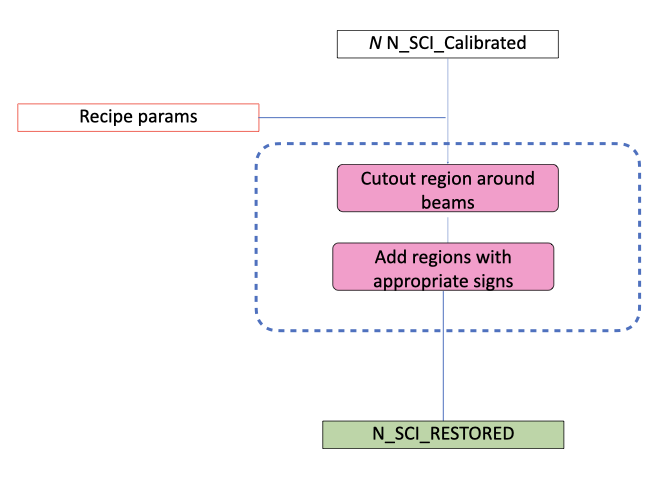
\includegraphics[width=0.9\textwidth]{metis_n_img_restore}
  \caption[Recipe: \REC*{metis_n_img_restore}]{\REC*{metis_n_img_restore} --
    Create a single positive image from chop-nod difference image}
  \label{fig:metis_n_img_restore}
\end{figure}

%%%%%%%%%%%%%%
\clearpage
\subsubsection{\REC*{metis_n_img_distortion}:  Distortion calibration}
\label{rec:metis_n_img_distortion}
\label{n_img_distortion}
\label{rec:n_img_distortion}
\label{sssec:n_img_distortion}

Calibration of the imaging distortion is done on an image of a pin
hole mask located in a focal plane within the instrument. The
distortion is described in terms of a polynomial model whose
coefficients can be transformed to WCS keywords and applied to any
other pipeline product. In addition to the distortion table, a map of
pixel scale across the detector will be created.

\begin{recipedef}
  Name:                & \REC{metis_n_img_distortion}                                   \\
  Purpose:             & Determine optical distortion coefficients for the N imager.    \\
  Templates:           & \TPL{METIS_img_n_cal_distortion}                               \\
  Type:                & Calibration                                                    \\
  Input data:          & \RAW{N_DISTORTION_RAW} (Images of grid mask in WCU-FP2 or CFO-FP2.)\\
                       & \RAW{N_WCU_OFF_RAW} \\
                       & \EXTCALIB{PINHOLE_TABLE} (Grid of pinhole mask positions) \\
%                       & \PROD{BADPIX_MAP_GEO} \\
  Matched keywords:    & \FITS{DRS.FILTER} \\
  Parameters:          & Parameters for fitting routine \\
  Algorithm:           & Subtract background image.  (\CODE{hdrl_imagelist_sub_image})                                       \\
                       & Measure location of point source images in frames.   (\CODE{hdrl_catalogue_create})            \\
                       & call \DRL{fit_distortion} to fit polynomial coefficients to deviations from grid positions. \\
  Output data:         & \PROD{N_DISTORTION_TABLE} \\
                       & \PROD{N_DISTORTION_MAP}        \\
                       & \PROD{N_DIST_REDUCED}             \\
  Expected accuracies: & $2\times 10^{-3}$ (cf.~\cite{METIS_calerrbudget})                                                            \\
  QC1 parameters:      & \QC{QC N DISTORT RMS}                                          \\
                       & \QC{QC N DISTORT NSOURCE}  \\
  hdrl functions:      & \CODE{hdrl_catalogue_create}                                   \\
                       & \CODE{hdrl_imagelist_sub_image}                                \\
\end{recipedef}

\begin{figure}[hb]
    \centering
    \def \globalscale {0.700000}
    \fontsize{10}{12}\selectfont
    % % Document preamble. Comment out for final figure! Footer too!
% \documentclass[tikz, margin=5mm, dvipsnames]{standalone}
% \usepackage{hyperref}
% \usepackage{listings}
% 
% ADDING NEW DEFINITIONS -------------------------------------------- start
\definecolor{listingbg}{gray}{0.95}
\definecolor{darkgreen}{rgb}{0.0, 0.7, 0.0}
\definecolor{darkblue} {rgb}{0.0, 0.0, 0.7}
\definecolor{cyan} {rgb}{0.0, 0.4, 0.4}
\definecolor{darkred}  {rgb}{0.7, 0.0, 0.0}
\definecolor{darkorange}{rgb}{1.0, 0.49, 0.0}
\definecolor{violett}{rgb}{255, 0, 255}
\definecolor{turq}{rgb}{0.0, 0.7, 0.8}
\definecolor{fits}{rgb}{0.4, 0.1, 1}


\makeatletter
\lstdefinestyle{RAWstyle}{%
  basicstyle=\ttfamily\color{black}%
  \lst@ifdisplaystyle\scriptsize\fi}

\lstdefinestyle{PARstyle}{%
  basicstyle=\ttfamily\color{black}%
  \lst@ifdisplaystyle\scriptsize\fi}

\lstdefinestyle{DRLstyle}{%
  basicstyle=\ttfamily\color{black}%
  \lst@ifdisplaystyle\scriptsize\fi}

\lstdefinestyle{RECstyle}{%
  basicstyle=\ttfamily\color{black}%
  \lst@ifdisplaystyle\scriptsize\fi}

\lstdefinestyle{QCstyle}{%
  basicstyle=\ttfamily\color{black}%
  \lst@ifdisplaystyle\scriptsize\fi}

\lstdefinestyle{TPLstyle}{%
  basicstyle=\ttfamily\color{black}%
  \lst@ifdisplaystyle\scriptsize\fi}

\lstdefinestyle{PRODstyle}{%
  basicstyle=\ttfamily\color{black}%
  \lst@ifdisplaystyle\scriptsize\fi}

\lstdefinestyle{EXTCALIBstyle}{%
  basicstyle=\ttfamily\color{black}%
  \lst@ifdisplaystyle\scriptsize\fi}

\lstdefinestyle{STATCALIBstyle}{%
  basicstyle=\ttfamily\color{black}%
  \lst@ifdisplaystyle\scriptsize\fi}
\makeatother

% \makeatletter
\newcommand{\replaceunderscores}[1]{\expandafter\replace@underscores#1_\relax}

\def\replace@underscores#1_#2\relax{%
    \ifx \relax #2\relax
        #1%
    \else
        #1%
        \textunderscore
        \replace@underscores#2\relax
    \fi
}

\ExplSyntaxOn
% Generic \Smart@Item macro:
%   use \NEWRAW*{WHATEVER_THIS_IS} where hyperlinks are not needed (TOC, sections...)
%   and \NEWRAW{WHATEVER_THIS_IS} for a full hyperlink-enabled version in regular text and tikz figures
\NewDocumentCommand{\Smart@Item}{m m m O{dataitem}}{%
    \IfBooleanTF{#1}{%
        \texorpdfstring{\lstinline[style=#2style]!#3!}{\replaceunderscores{#3}}%
    }{%
        \hyperref[#4:\text_lowercase:n{#3}]{\lstinline[style=#2style]!#3!}%
    }%
}
\ExplSyntaxOff

% Raw FITS file: \NEWRAW{LM_SCI_RAW}
\NewDocumentCommand{\NEWRAW}{s m}{\Smart@Item{#1}{RAW}{#2}}
\NewDocumentCommand{\NEWPAR}{s m}{\Smart@Item{#1}{PAR}{#2}}
\NewDocumentCommand{\NEWDRL}{s m}{\Smart@Item{#1}{DRL}{#2}}
\NewDocumentCommand{\NEWREC}{s m}{\Smart@Item{#1}{REC}{#2}[rec]}
\NewDocumentCommand{\NEWQC}{s m}{\Smart@Item{#1}{QC}{#2}}
\NewDocumentCommand{\NEWTPL}{s m}{\Smart@Item{#1}{TPL}{#2}}
\NewDocumentCommand{\NEWPROD}{s m}{\Smart@Item{#1}{PROD}{#2}}
\NewDocumentCommand{\NEWREQ}{s m}{\Smart@Item{#1}{REQ}{#2}}
\NewDocumentCommand{\NEWEXTCALIB}{s m}{\Smart@Item{#1}{EXTCALIB}{#2}}
\NewDocumentCommand{\NEWSTATCALIB}{s m}{\Smart@Item{#1}{STATCALIB}{#2}}
\NewDocumentCommand{\NEWFITS}{s m}{\Smart@Item{#1}{FITS}{#2}}
\makeatother

%% Write DRL functions names like this: \hyperref[drl:function]{\DRL{function}}
\newcommand{\RAW}[1]{ \texorpdfstring{\lstinline[style=RAWstyle]!#1!}%
                                     {\replaceunderscores{#1}}}

%% Write DRL functions names like this: \hyperref[drl:function]{\DRL{function}}
\newcommand{\PAR}[1]{ \texorpdfstring{\lstinline[style=PARstyle]!#1!}%
                                     {\replaceunderscores{#1}}}

%% Write DRL functions names like this: \hyperref[drl:function]{\DRL{function}}
\newcommand{\DRL}[1]{ \texorpdfstring{\lstinline[style=DRLstyle]!#1!}%
                                     {\replaceunderscores{#1}}}

%% Write recipe names like this: \REC{metis_do_stuff}
\newcommand{\REC}[1]{ \texorpdfstring{\lstinline[style=RECstyle]!#1!}%
                                     {\replaceunderscores{#1}}}

%% Write QC parameters like this: \QC{QC_SOMETHING_OR_OTHER}
\newcommand{\QC}[1]{ \texorpdfstring{\lstinline[style=QCstyle]!#1!}%
                                    {\replaceunderscores{#1}}}

%% Write templates like this: \TPL{DARK_LM}
\newcommand{\TPL}[1]{ \texorpdfstring{\lstinline[style=TPLstyle]!#1!}%
                                     {\replaceunderscores{#1}}}

%% Write products like this: \hyperref[dataitem:some_thing]{\PROD{SOME_THING}}
\newcommand{\PROD}[1]{ \texorpdfstring{\lstinline[style=PRODstyle]!#1!}%
                                      {\replaceunderscores{#1}}}

%% Write requirements like this: \REQ{METIS-xxxx}
\newcommand{\REQ}[1]{\href{https://polarion.astron.nl/polarion/\#/project/METIS/workitem?id=#1}{\textcolor{brown}{#1}}}

%% external calib files
\newcommand{\EXTCALIB}[1]{ \texorpdfstring{\lstinline[style=EXTCALIBstyle]!#1!}%
                                          {\replaceunderscores{#1}}}

% static calib files
\newcommand{\STATCALIB}[1]{ \texorpdfstring{\lstinline[style=STATCALIBstyle]!#1!}%
                                           {\replaceunderscores{#1}}}

%% Write FITS keywords (and values) like this: \FITS{EXPTIME}
\newcommand{\FITS}[1]{ \texorpdfstring{\lstinline[]!#1!}%
                                      {\replaceunderscores{#1}}}


% \begin{document}



% ADDING NEW DEFINITIONS -------------------------------------------- start
\definecolor{listingbg}{gray}{0.95}
\definecolor{darkgreen}{rgb}{0.0, 0.7, 0.0}
\definecolor{darkblue} {rgb}{0.0, 0.0, 0.7}
\definecolor{cyan} {rgb}{0.0, 0.4, 0.4}
\definecolor{darkred}  {rgb}{0.7, 0.0, 0.0}
\definecolor{darkorange}{rgb}{1.0, 0.49, 0.0}
\definecolor{violett}{rgb}{255, 0, 255}
\definecolor{turq}{rgb}{0.0, 0.7, 0.8}
\definecolor{fits}{rgb}{0.4, 0.1, 1}


\makeatletter
\lstdefinestyle{RAWstyle}{%
  basicstyle=\ttfamily\color{black}%
  \lst@ifdisplaystyle\scriptsize\fi}

\lstdefinestyle{PARstyle}{%
  basicstyle=\ttfamily\color{black}%
  \lst@ifdisplaystyle\scriptsize\fi}

\lstdefinestyle{DRLstyle}{%
  basicstyle=\ttfamily\color{black}%
  \lst@ifdisplaystyle\scriptsize\fi}

\lstdefinestyle{RECstyle}{%
  basicstyle=\ttfamily\color{black}%
  \lst@ifdisplaystyle\scriptsize\fi}

\lstdefinestyle{QCstyle}{%
  basicstyle=\ttfamily\color{black}%
  \lst@ifdisplaystyle\scriptsize\fi}

\lstdefinestyle{TPLstyle}{%
  basicstyle=\ttfamily\color{black}%
  \lst@ifdisplaystyle\scriptsize\fi}

\lstdefinestyle{PRODstyle}{%
  basicstyle=\ttfamily\color{black}%
  \lst@ifdisplaystyle\scriptsize\fi}

\lstdefinestyle{EXTCALIBstyle}{%
  basicstyle=\ttfamily\color{black}%
  \lst@ifdisplaystyle\scriptsize\fi}

\lstdefinestyle{STATCALIBstyle}{%
  basicstyle=\ttfamily\color{black}%
  \lst@ifdisplaystyle\scriptsize\fi}
\makeatother

%%% This file contains definitions of shapes and nodes used
%%% for a recipe workflow
%%% Author       : Oliver Czoske
%%% Created      : 2021-03-03
%%% Last Changed : 2021-03-03
%%% Changes:
%%%

\usetikzlibrary{
  shapes.misc,
  positioning,
  calc,
  arrows.meta}

%% All connecting lines have an arrow
\tikzset{
  connection_arrow/.style={->, >=Latex[open], thick}
}

%% Start and stop buttons (black disks, stop with ring)
%% These are pics, use as
%%         \pic (name) [above of=..] {picname};
\tikzset{
  start/.pic = {
    \node (-m) at (0, 0){};
    \filldraw [fill=black] (0, 0) circle (0.2);
  }
}

\tikzset{
  stop/.pic = {
    \node (-m) at (0, 0){};
    \node (-t) at (0, -0.3){};
    \filldraw [fill=black] (0, 0) circle(0.2);
    \draw[black] (0, 0) circle (0.3);
  }
}


%%%% Various boxes and their colours
%%%% These are nodes, use as
%%%% \node (name) [type, location]  {text};

\definecolor{stepcolor}{RGB}{210,169,188}
\definecolor{rawcolor}{RGB}{205,205,205}
\definecolor{externalcolor}{RGB}{183,255,255}
\definecolor{calibcolor}{RGB}{255,250,216}
\definecolor{calproductcolor}{RGB}{185,184,237}
\definecolor{qcproductcolor}{RGB}{255,201,165}
\definecolor{sciproductcolor}{RGB}{197,219,183}
\definecolor{framecolor}{RGB}{127,13,65}

\tikzset{
  %% template : the template(s) that trigger(s) the recipe
  template/.style={
    rectangle,
    draw=black,
    minimum width=4.0cm,
    minimum height=0.5cm,
    align=center
  },
  %% input : the input files
  input/.style={
    rectangle,
    fill=rawcolor,
    minimum width=4.0cm,
    minimum height=0.75cm,
%     text width=3cm,
    align=center
  },
  %% calib : calibration input
  calib/.style={
    rectangle,
    fill=calibcolor,
    minimum width=4.0cm,
    minimum height=0.75cm,
%     text width=3cm,
    align=center
  },
  %% external : external input
  external/.style={
    rectangle,
    fill=externalcolor,
    minimum width=4.0cm,
    minimum height=0.75cm,
%     text width=3.5cm,
    align=center
  },
  %% params : parameters
  params/.style={
    rectangle,
    draw=red,
    thick,
    minimum width=4.0cm,
    minimum height=0.75cm,
%     text width=3cm,
    align=center
  },
  %% redstep : a reduction step
  %%      ("step" is predefined and can't be used)
  redstep/.style={
    rectangle,
    rounded corners=0.2cm,
    fill=stepcolor,   %%% define colour!
    minimum width=4.0cm,
    minimum height=1cm,
%     text width=3cm,
    align=center
  },
  %% connection : connection to input or output
  connection/.style={
    circle,
    fill=black,
    minimum size=0.15cm,
    inner sep=0pt
  },
  %% sciproduct : a science product
  sciproduct/.style={
    rectangle,
    fill=sciproductcolor,
    minimum width=4.0cm,
    minimum height=0.75cm,
%     text width=3.5cm,
    align=center
  },
  %% calproduct : a calibration product
  calproduct/.style={
    rectangle,
    fill=calproductcolor,
    minimum width=4.0cm,
    minimum height=0.75cm,
%     text width=3.5cm,
    align=center
  },
  %% frame : frame around the recipe
  %% This is a path, use as
  %%    \draw [frame] (upper left) rectangle (lower right);
  frame/.style={framecolor, very thick, dashed}
}


\begin{tikzpicture}
  [x=1cm,
  y=-1cm,
  align=center,
  node distance=2cm and 3cm]
  \sffamily

  %% Grid for orientation. Comment out for final figure!
  % \draw[help lines, green](-5, 0) grid (8, 11);

  %%% Put workflow commands here:
  %% Main reduction workflow

%  \node (template) [template]{%
%    METIS\_img\_n\_cal\_distortion};

  \pic (start) {start};

  \node (input) [below=0.75cm of start-m, input] {%
    \hyperref[dataitem:n_distortion_raw]{\RAW{N_DISTORTION_RAW}}
  };

  \node (step_subtract) [below=2.5cm of input, redstep]{%
    subtract WCU OFF dark
  };

  \node (step_locate) [below=2.5cm of step_subtract, redstep]{%
    locate images};

  \node (step_fit) [below=1.5cm of step_locate, redstep]{%
    fit polynomial};

  \pic (stop) [below=3cm of step_fit]{stop};

  %% Input
  \node (connect_wcuoff) [connection] at
  ($(input)!0.65!(step_subtract)$) {};
  \node (wcuoff) [left=of connect_wcuoff, input] {\hyperref[dataitem:n_wcu_off_raw]{\RAW{N_WCU_OFF_RAW}}};
  \draw (wcuoff) -- (connect_wcuoff);

  \node (connect_bpmin) [connection] at
  ($(step_subtract)!0.3!(step_locate)$) {};
  \node (bpmin) [left=of connect_bpmin, calproduct] {\hyperref[dataitem:badpix_map_geo]{\STATCALIB{BADPIX_MAP_GEO}}};
  \draw (bpmin) -- (connect_bpmin);

  \node (connect_pinhole) [connection] at
  ($(step_subtract)!0.7!(step_locate)$) {};
  \node (pinhole) [left=of connect_pinhole, external] {\hyperref[dataitem:pinhole_table]{\EXTCALIB{PINHOLE_TABLE}}};
  \draw (pinhole) -- (connect_pinhole);

  %% Connections
  \draw (start-m) -- (input);
  \draw (input) -- (step_subtract);
  \draw (step_subtract) -- (step_locate);
  \draw (step_locate) -- (step_fit);
  \draw (step_fit) -- (stop-t);

  %% Output
  \node (connectdisttable) [connection] at
  ($(step_fit)!0.25!(stop-t)$) {};
  \node (disttable) [right=of connectdisttable, calproduct, minimum width=4cm]{%
    \hyperref[dataitem:n_distortion_table]{\STATCALIB{N_DISTORTION_TABLE}}};
  \draw (connectdisttable) -- (disttable);

  \node (connectdistmap) [connection] at
  ($(step_fit)!0.5!(stop-t)$) {};
  \node (distmap) [right=of connectdistmap, calproduct, minimum width=4cm]{%
    \hyperref[dataitem:n_distortion_map]{\STATCALIB{N_DISTORTION_MAP}}};
  \draw (connectdistmap) -- (distmap);

  \node (connectdistreduced) [connection] at
  ($(step_fit)!0.75!(stop-t)$) {};
  \node (distreduced) [right=of connectdistreduced, calproduct, minimum width=4cm]{%
    \hyperref[dataitem:n_dist_reduced]{\PROD{N_DIST_REDUCED}}};
  \draw (connectdistreduced) -- (distreduced);

  %% Frame around recipe
  \draw [frame]
  ($(input)!0.25!(step_subtract) - (2.75,0)$) rectangle
  ($(step_fit)!0.85!(stop-t) + (2.5,0)$);
  \node [framecolor, anchor=north west] at
  ($(input)!0.25!(step_subtract) - (2.75, 0)$){%
    \textsl{metis\_n\_img\_distortion}};

\end{tikzpicture}

% ADDING NEW DEFINITIONS -------------------------------------------- start
\definecolor{listingbg}{gray}{0.95}
\definecolor{darkgreen}{rgb}{0.0, 0.7, 0.0}
\definecolor{darkblue} {rgb}{0.0, 0.0, 0.7}
\definecolor{cyan} {rgb}{0.0, 0.4, 0.4}
\definecolor{darkred}  {rgb}{0.7, 0.0, 0.0}
\definecolor{darkorange}{rgb}{1.0, 0.49, 0.0}
\definecolor{violet}{rgb}{255, 0, 255}
\definecolor{turq}{rgb}{0.0, 0.7, 0.8}
\definecolor{fits}{rgb}{0.4, 0.1, 1}


\makeatletter
\lstdefinestyle{RAWstyle}{%
  basicstyle=\ttfamily\color{fits}%
  \lst@ifdisplaystyle\scriptsize\fi}

\lstdefinestyle{PARstyle}{%
  basicstyle=\ttfamily\color{cyan}%
  \lst@ifdisplaystyle\scriptsize\fi}

\lstdefinestyle{DRLstyle}{%
  basicstyle=\ttfamily\color{violet}%
  \lst@ifdisplaystyle\scriptsize\fi}

\lstdefinestyle{RECstyle}{%
  basicstyle=\ttfamily\color{darkgreen}%
  \lst@ifdisplaystyle\scriptsize\fi}

%% Write QC parameters like this: \QC{QC_SOMETHING_OR_OTHER}
\lstdefinestyle{QCstyle}{%
  basicstyle=\ttfamily\color{darkblue}%
  \lst@ifdisplaystyle\scriptsize\fi}

%% Write templates like this: \TPL{DARK_LM}
\lstdefinestyle{TPLstyle}{%
  basicstyle=\ttfamily\color{darkred}%
  \lst@ifdisplaystyle\scriptsize\fi}

%% Write products like this: \hyperref[dataitem:some_thing]{\PROD{SOME_THING}}
\lstdefinestyle{PRODstyle}{%
  basicstyle=\ttfamily\color{darkorange}%
  \lst@ifdisplaystyle\scriptsize\fi}

%% external calib files
\lstdefinestyle{EXTCALIBstyle}{%
  basicstyle=\ttfamily\color{Turquoise}%
  \lst@ifdisplaystyle\scriptsize\fi}

% static calib files
\lstdefinestyle{STATCALIBstyle}{%
  basicstyle=\ttfamily\color{teal}%
  \lst@ifdisplaystyle\scriptsize\fi}
\makeatother



% % Document footer. Comment out for final figure! Header too!
% \end{document}

  \caption[Recipe: \REC*{metis_n_img_distortion}]{%
    \REC{metis_n_img_distortion} -- \CODE{IMG_N} distortion calibration}
  \label{fig:metis_n_img_distortion}
\end{figure}

%%% Local Variables:
%%% TeX-master: "METIS_DRLD"
%%% End:
